\documentclass[journal,12pt,twocolumn]{IEEEtran}
\usepackage{amsmath}
\usepackage{amssymb}
\usepackage{enumerate}
\usepackage[utf8]{inputenc}
\usepackage{multicol}
\usepackage{gensymb}
\usepackage{mathtools}
%\usepackage{graphicx}
\usepackage{iithtlc}
%\usepackage{iithquiz}

\graphicspath{ {/home/theresh/Desktop/DSP} }



\newcommand\Mycomb[2][^n]{\prescript{#1\mkern-0.5mu}{}C_{#2}}


\begin{document}
\providecommand{\qfunc}[1]{\ensuremath{Q\left(#1\right)}}
\providecommand{\sbrak}[1]{\ensuremath{{}\left[#1\right]}}
\providecommand{\lsbrak}[1]{\ensuremath{{}\left[#1\right.}}
\providecommand{\rsbrak}[1]{\ensuremath{{}\left.#1\right]}}
\providecommand{\brak}[1]{\ensuremath{\left(#1\right)}}
\providecommand{\lbrak}[1]{\ensuremath{\left(#1\right.}}
\providecommand{\rbrak}[1]{\ensuremath{\left.#1\right)}}
\providecommand{\cbrak}[1]{\ensuremath{\left\{#1\right\}}}
\providecommand{\lcbrak}[1]{\ensuremath{\left\{#1\right.}}
\providecommand{\rcbrak}[1]{\ensuremath{\left.#1\right\}}}

\title{
\logo{Gate problems in DSP
%\logo{Gate problems in DSP}{\includegraphics[scale=0.3]{tlc2.eps}}{}{}
}
}

\maketitle

\begin{abstract}
These problems have been selected from
GATE question papers and can be used for conducting
tutorials in courses related to the course Digital Signal Processing in practice.
\end{abstract}


\begin{enumerate}
\setlength\itemsep{2em}

\item If the impulse response of a discrete-time system is $h[n]=-5^{n}u[-n-1]$,then the system function $H(z)$ is equal to
\begin{enumerate}[(A)]

\setlength\itemsep{1em}

\item $\frac{-z}{z-5}$ and the system is stable
\item $
\frac{z}{z-5}$ and the system is stable

\item $
\frac{-z}{z-5}$ and the system is unstable

\item $
\frac{z}{z-5}$ and the system is unstable

\end{enumerate}

%\item In below figure, $m(t)=\frac{2sin 2\pi t}{t}$,$s(t)=cos200\pi t$ and $n(t)=\frac{sin199\pi t}{t}$.The output is \\
%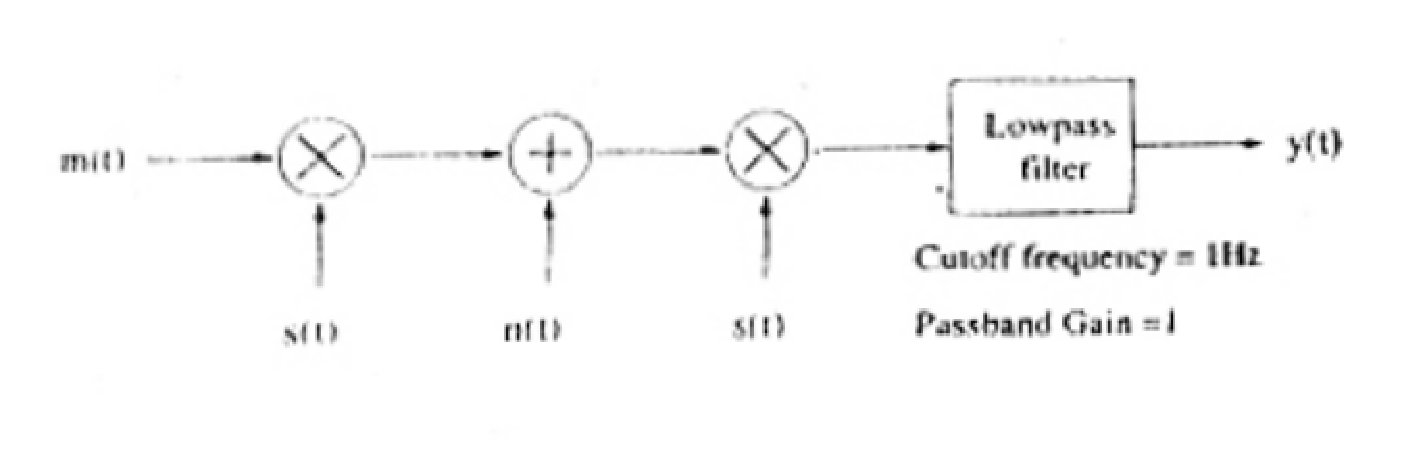
\includegraphics[scale=0.45]{fig20.eps}
%\begin{enumerate}[(A)]
%\setlength\itemsep{1em}
%\item $
%\frac{sin 2\pi t}{t}
%$
%\item $
%\frac{sin 2\pi t}{t}+\frac{sin 2\pi t}{t}cos(3 \pi t)
%$
%\item $
%\frac{sin 2\pi t}{t}+\frac{sin 0.5\pi t}{t}cos(1.5 \pi t)
%$
%\item $
%\frac{sin 2\pi t}{t}+\frac{sin \pi t}{t}cos(0.75 \pi t)
%$
%
%\end{enumerate}

%\item A signal $x(t)=100 cos(24 \pi \times 10^{3}t)$ is ideally sampled with a sampling period of 50$\mu$sec and then passed through an ideal low-pass filter with cutoff frequency of 15 KHz. Which of the following frequencies is/are present at the filter output ?
%
%\begin{enumerate}[(A)]
%\begin{multicols}{2}
%\setlength\itemsep{1em}
%\item 
%12 KHz only
%
%\item 8 KHz only
%\item 12 KHz and 9 KHz
%
%
%\item 12 KHz and 8 KHz
%
%
%\end{multicols}
%\end{enumerate}

%\item The Fourier series expansion of a real periodic signal with fundamental frequency $f_0$ is given by $g_p(t)=\sum\limits_{n=-\infty}^{+\infty} c_n e^{j2\pi n f_0 t}$ is is given that $C_3=3+j5$.Then $C_{-3}$ is
%\begin{enumerate}[(A)]
%\begin{multicols}{2}
%\setlength\itemsep{1em}
%\item $
%5+j3
%$
%\item $
%-3-j5
%$
%\item $
%-5-j3
%$
%\item $
%3-j5
%$
%\end{multicols}
%\end{enumerate}

%\item Let $x(t)$ be the input to a linear,time-invariant system. The required output is $4x(t-2)$.The transfer function of the system should be
%\begin{enumerate}[(A)]
%\begin{multicols}{4}
%\setlength\itemsep{1em}
%\item $
%4e^{j4\pi f}
%$
%\item $
%2e^{-j8\pi f}
%$
%\item $
%4e^{-j4\pi f}
%$
%\item $
%2e^{j8\pi f}
%$
%\end{multicols}
%\end{enumerate}
%


\item A sequence $x(n)$ with the z-transform $X(z)=z^{4}+z^{2}-2z+2-3z^{-4}$ is applied as an input to a linear,time-invariant system with the impulse response $h(n)=2\delta(n-3)$ where
\[
	\delta(n)=\begin{cases}
		1, & \text{if n=0 }  \\
		0, & \text{otherwise }\,.
	\end{cases}
\]
The output at $n$=4 is
\begin{enumerate}[(A)]
\begin{multicols}{4}
\setlength\itemsep{1em}
\item $
-6
$
\item $
0
$
\item $
2
$
\item $
-4
$
\end{multicols}
\end{enumerate}

% 2003 67
%\item Let $x(t)=2cos(800\pi t)+cos(1400\pi t)$,$x(t)$ sampled with the rectangular pulse train shown in figure. The only spectral components (in kHz) present in the sampled signal in the frequency range 2.5 kHz to 3.5 kHz are \\
%
%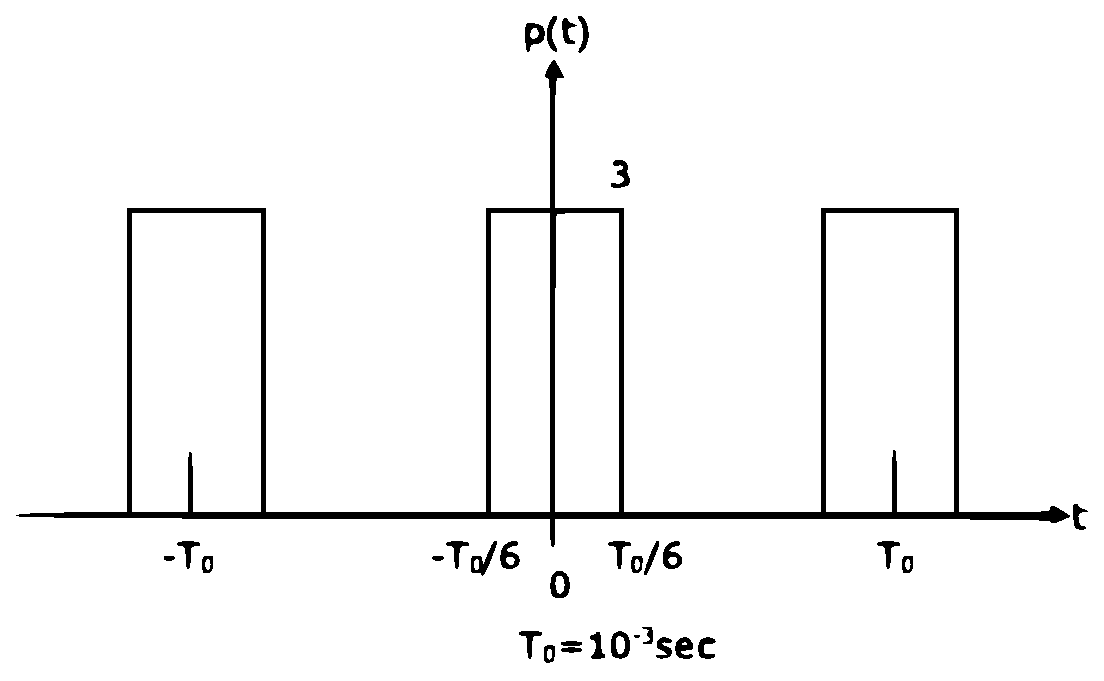
\includegraphics[scale=0.4]{fig2.eps}\\
%
%\begin{enumerate}[(A)]
%\begin{multicols}{2}
%\setlength\itemsep{1em}
%\item $
%2.7,3.4
%$
%\item $
%3.3,3.6
%$
%\item $
%2.6,2.7,3.3,3.4,3.6
%$
%\item $
%2.7,3.3
%$
%\end{multicols}
%\end{enumerate}

Data for \textbf{\textit{Q.3-4 }} are given below. Solve the problems and choose the correct answers.\newline The system under consideration is an RC low-pass filter (RC-LPF) with R=1.0K$\Omega$ and C=1.0 $\mu$F

\item Let $H(f)$ denote the frequency response of the RC-LPF. Let $f_1$ be the highest frequency such that $0\leq |f| \leq f_1$,$\frac{|H(f_1|}{H(0)}\geq 0.95$.Then $f_1$ (in HZ) is
\begin{enumerate}[(A)]
\begin{multicols}{4}
\setlength\itemsep{1em}
\item $
327.8
$
\item $
163.9
$
\item $
52.2
$
\item $
104.4
$
\end{multicols}
\end{enumerate}

%\item Let $t_g(f)$ be the group dealy function of the given RC-LPF and $f_2=100 Hz$.Then $t_g(f_2)$ in ms,is\\
%
%\begin{enumerate}[(A)]
%\begin{multicols}{4}
%\setlength\itemsep{1em}
%\item $ 0.717
%$
%\item $
%7.17
%$
%\item $
%71.7$
%\item $
%4.505$
%
%\end{multicols}
%\end{enumerate}

\item The impulse response $h[n]$ of a linear time-invariant system is given by $h[n]=u[n+3]+u[n-2]-2u[n-7]$ \newline where $u[n]$ is the unit step sequence.The above system is\\
\begin{enumerate}[(A)]
%\begin{multicols}{2}
\setlength\itemsep{1em}
\item 
Stable but not causal

\item 
Stable and Causal

\item 
Causal but unstable

\item 
Unstable and not Causal


%\end{multicols}
\end{enumerate}


\item The z-transform of a system is $H(z)=\frac{z}{z-0.2}$.If the ROC IS $|z|<0.2$, then the impulse response of the system is

\begin{enumerate}[(A)]
\begin{multicols}{2}
\setlength\itemsep{1em}

\item $(0.2)^{n}u[n]$
\item $(0.2)^{n}u[-n-1]$
\item $-(0.2)^{n}u[n]$
\item $-(0.2)^{n}u[-n-1]$

\end{multicols}
\end{enumerate}

%\item The Fourier transform of a conjugate symmetric function is always
%\begin{enumerate}[(A)]
%
%\setlength\itemsep{1em}
%\item real
%\item conjugate anti-symmetric
%\item real
%\item conjugate symmetric
%
%\end{enumerate}

%\item The gain margin for the system with open-loop transfer function $G(s)H(z)=\frac{2(1+z)}{s^{2}}$
%
%\begin{enumerate}[(A)]
%\begin{multicols}{4}
%\setlength\itemsep{1em}
%
%\item $\infty$
%\item 0
%\item 1
%\item $-\infty$
%
%\end{multicols}
%\end{enumerate}

%\item A 1 kHz sinusoidal signal is ideally sampled at 1500 samples/sec and the sampled signal is passed through an ideal low-pass filter with cut-off freuency 800 Hz.The output signal has the frequency ?
%
%
%
%\begin{enumerate}[(A)]
%\begin{multicols}{2}
%\item 0 Hz
%\item 0.75 kHz
%\item 0.5 kHz
%\item 0.25 kHz
%\end{multicols}
%\end{enumerate}

% ec 2004 61
%\item A rectangular pulse train s(t) as shown in figure,is convolved with the signal $cos^{2}(4\pi \times 10^{3})t$.
%
%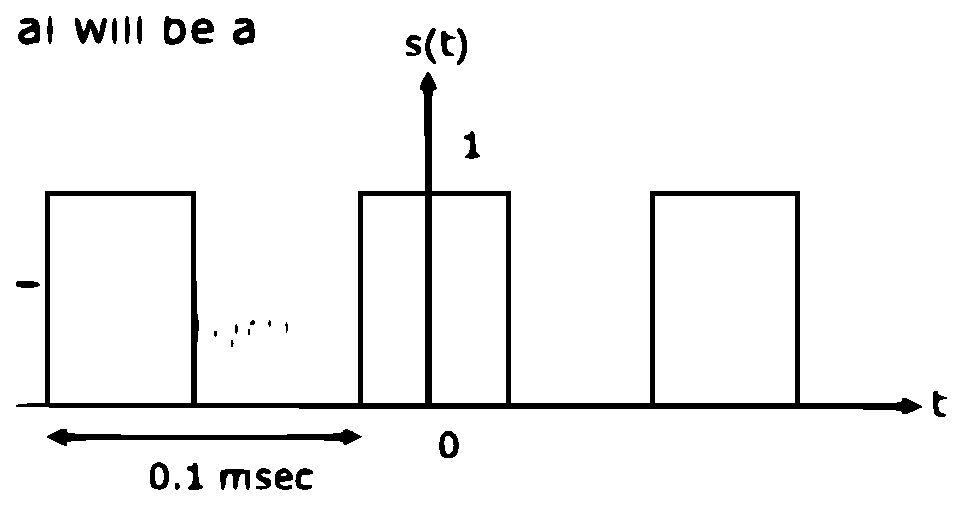
\includegraphics[scale=0.4]{fig3.eps}
%
%\begin{enumerate}[(A)]
%\begin{multicols}{2}
%\setlength\itemsep{1em}
%
%\item DC
%\item 12 kHz sinusoid
%\item 8 kHz sinusoid
%\item 14 kHz sinusoid
%\end{multicols}
%\end{enumerate}

\item consider the sequence $x[n]=[4-j5\hspace{2mm}1+j2 \hspace{2mm}4]$\newline The conjugate anti-symmetric part of the sequence is
\begin{enumerate}[(A)]

\setlength\itemsep{1em}
\item $
[-4-j2.5\hspace{4mm}j2 \hspace{4mm}4-j2.5]
$
\item $
[-j2.5\hspace{4mm}1\hspace{4mm}j2.5]
$
\item $
[-j5\hspace{4mm}j2 \hspace{4mm}0]
$
\item $
[-4\hspace{4mm}1 \hspace{4mm}4]
$

\end{enumerate}

\item A causal LTI system is described by the difference equation $2y[n]=ay[n-2]-2x[n]+bx[n-1]$ \newline the system is stable only if
\begin{enumerate}[(A)]

\setlength\itemsep{1em}
\item $|a|=2,|b|<2$
\item $|a|>2,|b|>2$
\item $|a|<2,$any value of b
\item $|b|<2,$ any value of a


\end{enumerate}

%\item A causal system having the transfer function $H(s)=\dfrac{1}{s+2}$ is excited with $10u(t)$.The time at which the ouput reaches $99\%$ of its steady state value is
%\begin{enumerate}[(A)]
%\begin{multicols}{2}
%\setlength\itemsep{1em}
%
%\item 2.7 sec
%\item 2.5 sec
%\item 2.4 sec
%\item 2.1 sec
%
%\end{multicols}
%\end{enumerate}





\item The impulse responce $h[n]$ of a linear time invariant system is given as
\[
	h[n]=\begin{cases}
		-2\sqrt{2}, & \text{if n=1,-1 }  \\
		4\sqrt{2}, & \text{n=2,-2 }\\
		0,&\text{otherwise}\,.
	\end{cases}
\] 
\newline If the input to the above system is the sequence $e^{\frac{jpn}{4}}$,then the ouput is

\begin{enumerate}[(A)]
\begin{multicols}{2}
\setlength\itemsep{1em}

\item $4\sqrt{2} e^{\frac{jpn}{4}}$
\item $4\sqrt{2} e^{\frac{-jpn}{4}}$
\item $4e^{\frac{jpn}{4}}$
\item $-4e^{\frac{jpn}{4}}$
\end{multicols}
\end{enumerate}

% ex 2005 5
%\item The function $x(t)$ is shown in figure. Even and odd parts of  a unit-step function $u(t)$ are respectively.\\
%
%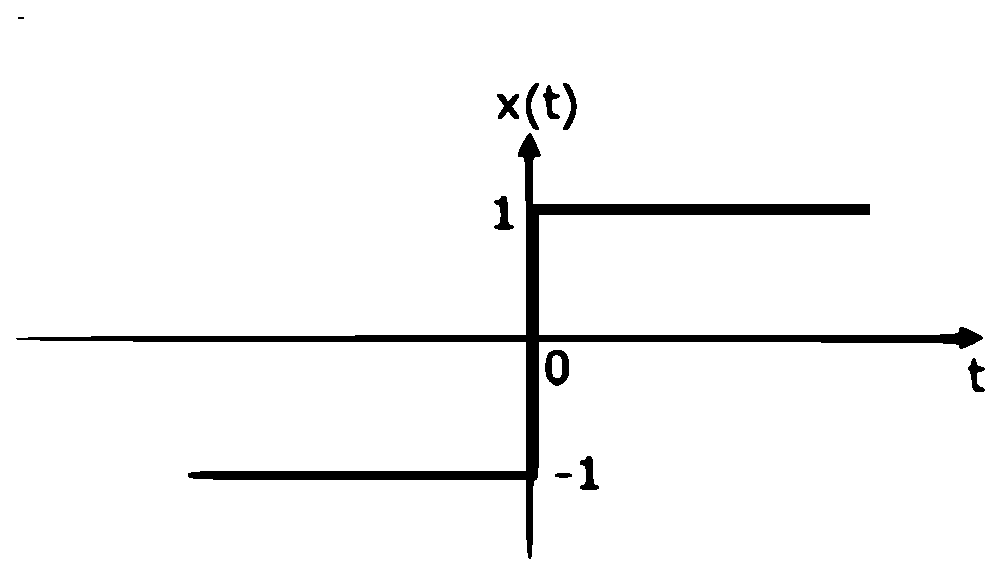
\includegraphics[scale=0.3]{fig4.eps}
%\begin{enumerate}[(A)]
%\begin{multicols}{2}
%\setlength\itemsep{1em}
%\item $
%\dfrac{1}{2},\dfrac{1}{2}x(t)
%$
%\item $-\dfrac{1}{2},\dfrac{1}{2}x(t)$
%\item $
%\dfrac{1}{2},-\dfrac{1}{2}x(t)
%$
%\item $
%-\dfrac{1}{2},-\dfrac{1}{2}x(t)
%$
%\end{multicols}
%\end{enumerate} 

\item The region of convergence of Z-transform of the sequence $(\frac{5}{6})^{n}u(n)-(\frac{6}{5})^{n}u(-n-1)$ must be
\begin{enumerate}[(A)]
\begin{multicols}{2}
\setlength\itemsep{1em}
\item $|z|<\frac{5}{6}$
\item $|z|>\frac{6}{5}$
\item $\frac{5}{6}<|z|<\frac{5}{6}$
\item $\frac{6}{5}<|z|<\infty$

\end{multicols}
\end{enumerate}

%ec 2005 20
%\item Which of the following can be impulse response of causal system ?\\
%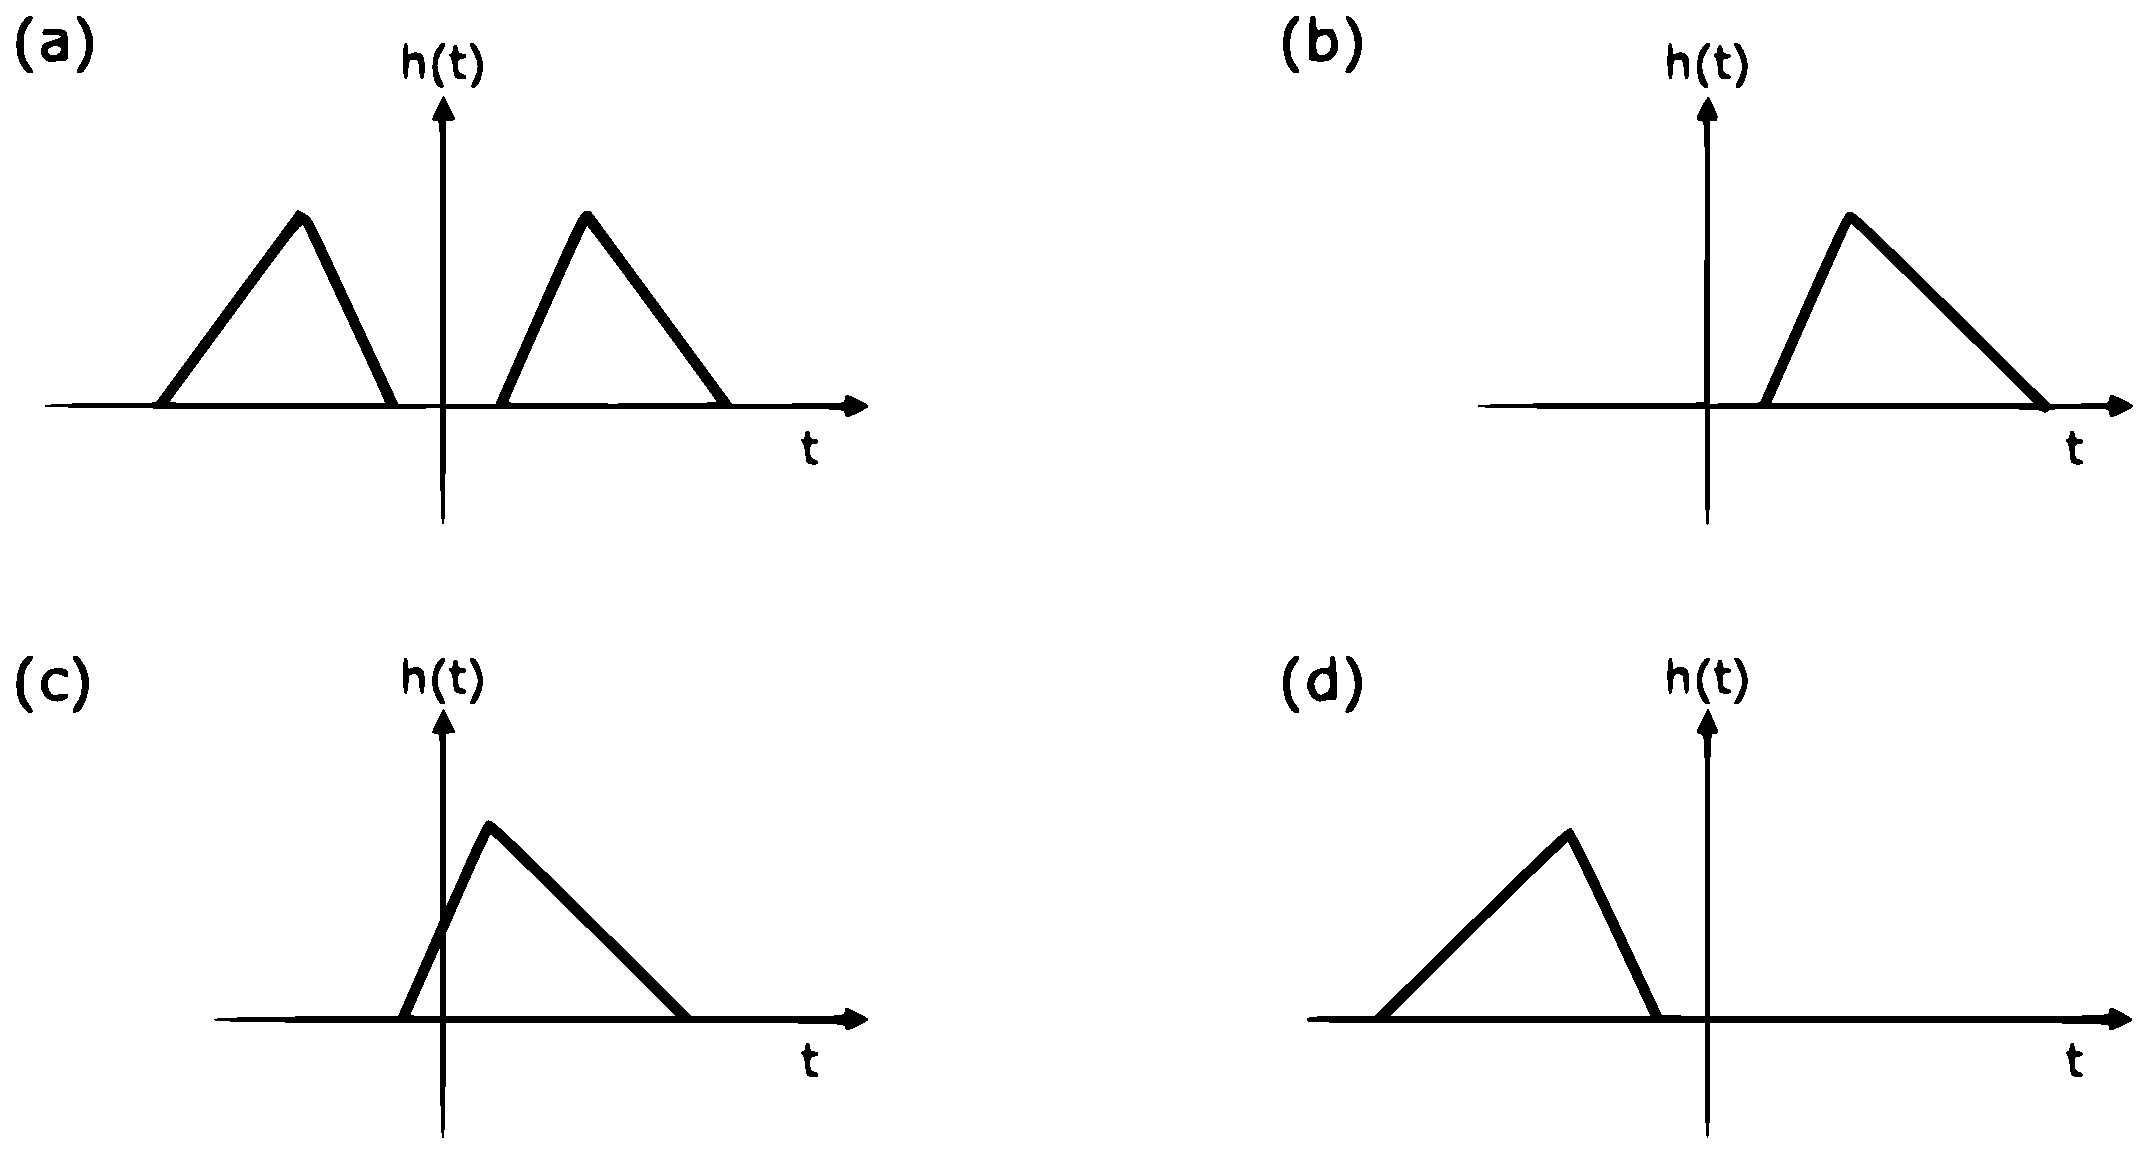
\includegraphics[scale=0.2]{fig5.eps}
%
%\item Let  $x(n)=(\frac{1}{2})^{n}, y(n)= x^{2}(n)$ and $Y(e^{jw})$ be the fourier transform of $y(n)$. Then $Y(e^{j0})$
%\begin{enumerate}[(A)]
%\begin{multicols}{2}
%\setlength\itemsep{1em}
%\item $\frac{1}{4}$
%\item 2
%\item 4
%\item $\frac{4}{3}$
%
%\end{multicols}
%\end{enumerate}

%\item The output $y(t)$ of a linear time invariant system is related to its input $x(t)$ by the following equation. $y(t)=0.5x(t-t_d+T)+x(t-t_d)+0.5x(t-t_d-T)$. The filter transfer function $H(w)$ of such a system is given by
%
%\begin{enumerate}[(A)]
%
%\setlength\itemsep{1em}
%
%\item $
%(1+coswT)e^{-jwt_d}
%$
%\item $
%(1+0.5coswT)e^{-jwt_d}
%$
%\item $
%(1+coswT)e^{jwt_d}
%$
%\item $
%(1-0.5coswT)e^{-jwt_d}
%$
%
%\end{enumerate}

\item A signal $x(n)=sin(\omega_0n+\phi)$ is the input to a LTI system frequency response $H(e^{j\omega})$.If the ouput of the system is $Ax(n-n_0)$, then the most general form of $\angle H(e^{j\omega})$ will be

\begin{enumerate}[(A)]

\setlength\itemsep{1em}

\item $
-n_0\omega_0 + \beta 
$ for any arbitary real $\beta$
\item  $
- n_0\omega_0 + 2\pi k
$ for any arbitary integer k.
\item  $
n_0\omega_0 + 2\pi k
$ for any arbitary integer k.
\item $
- n_0\omega_0 + \phi
$

\end{enumerate}

%\item For a signal $x(t)$ the Fourier transform is $X(f)$.Then the inverse Fourier transform of $X(3f+2)$ is given by
%\begin{enumerate}[(A)]
%
%\setlength\itemsep{1em}
%
%\item $
%\dfrac{1}{2} x(\dfrac{1}{2})e^{j3\pi t}
%$ 
%\item $
%3 x(3t)e^{-j4\pi t}
%$ 
%\item  $
%\dfrac{1}{3} x(\dfrac{1}{3})e^{\dfrac{-j4\pi t}{3}}
%$ 
%\item $
%x(3t+2)
%$
%
%\end{enumerate}

%% ec 2005 85
%\item \textbf{\textit{(A)}} The Sequence \[
%	y(n)=\begin{cases}
%		x(\dfrac{n}{2}-1), & \text{for n even }  \\
%		0, & \text{odd }\,.
%	\end{cases}
%\] will be\\
%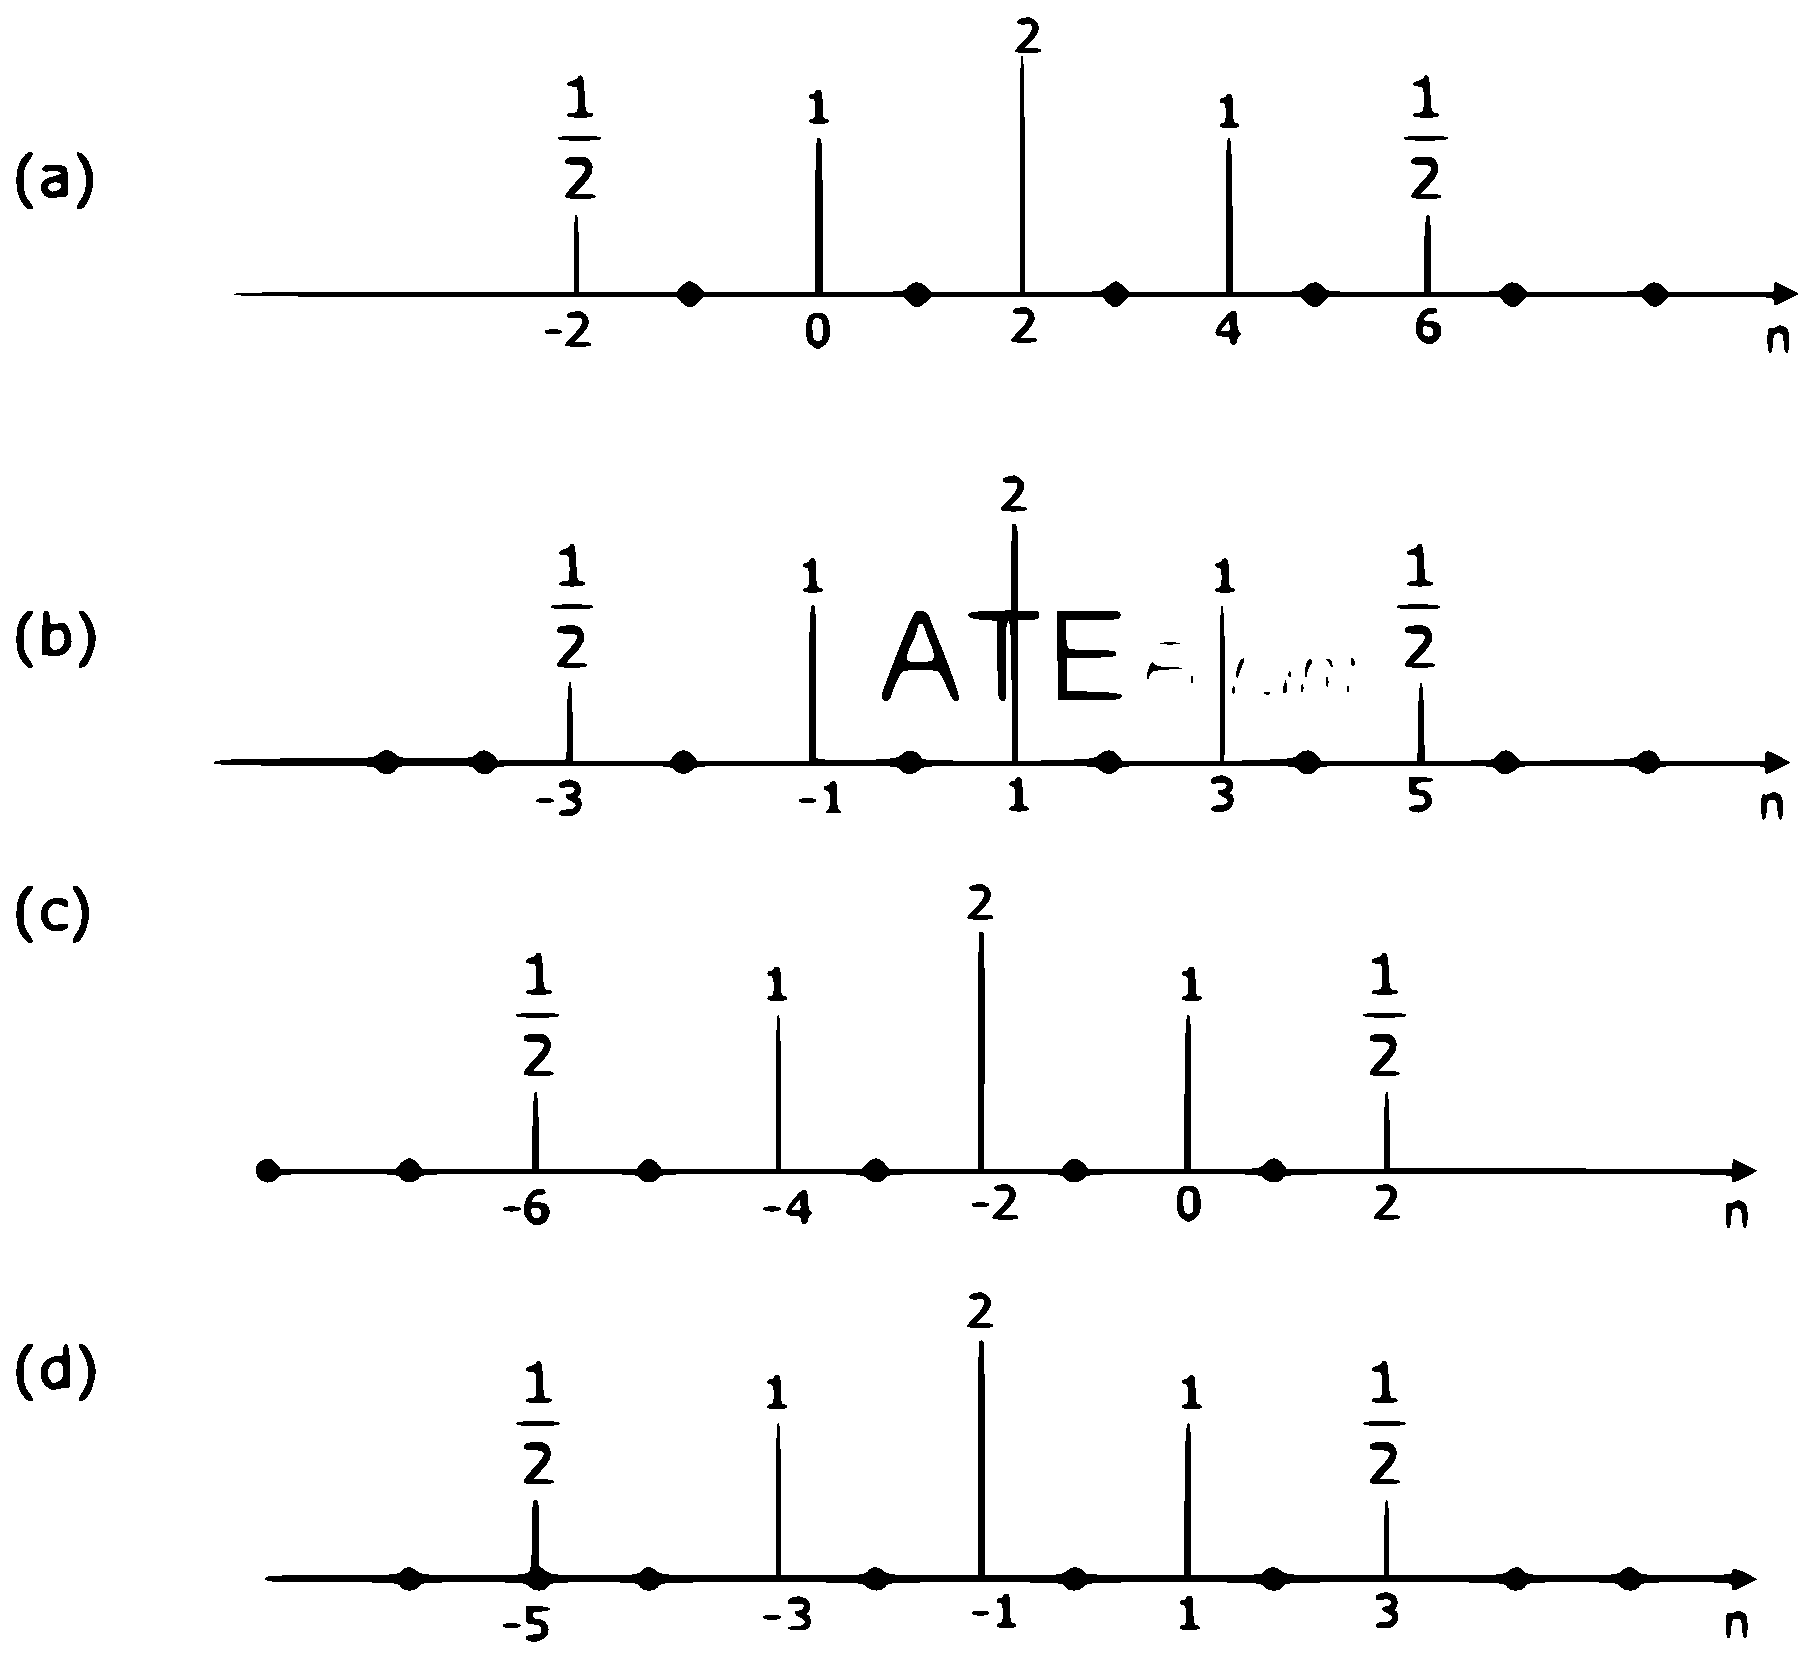
\includegraphics[scale=0.3]{fig6.eps}
%
%\textbf{\textit{(B)}} The Fourier transform of $y(2n)$ will be\\
%\begin{enumerate}[(A)]
%
%\setlength\itemsep{1em}
%
%\item $
%e^{-2j\omega}[cos 4\omega +2 cos 2\omega +2]
%$ 
%\item $
%[cos2\omega +2 cos\omega +2]
%$ 
%\item  $
%e^{-j\omega}[cos2\omega +2 cos\omega +2]
%$ 
%\item $
%e^{j\omega}[cos2\omega +2 cos\omega +2]
%$
%
%\end{enumerate}


%\item Let $x(t)\leftrightarrow X(j\omega)$ be Fourier Transform pair.The Fourier Transform of the signal $x(5t-3)$ in terms of $X(j\omega)$ is given as\\
%\begin{enumerate}[(A)]
%
%\setlength\itemsep{1em}
%
%\item $
%\dfrac{1}{5}e^{\dfrac{-j3\omega}{5}}X(\dfrac{j\omega}{5})
%$ 
%\item $
%\dfrac{1}{5}e^{\dfrac{j3\omega}{5}}X(\dfrac{j\omega}{5})
%$ 
%\item  $
%\dfrac{1}{5}e^{-j3\omega}X(\dfrac{j\omega}{5})
%$ 
%\item $
%\dfrac{1}{5}e^{j3\omega}X(\dfrac{j\omega}{5})
%$
%
%\end{enumerate}




%\item The dirac delta function $\delta(t)$ is defined as
%
%\begin{enumerate}[(A)]
%
%\setlength\itemsep{1em}
%
%\item \[
%	\delta(t)=\begin{cases}
%		1, & \text{t=0}  \\
%		0, & \text{otherwise }\,.
%	\end{cases}
%\]
%\item \[
%	\delta(t)=\begin{cases}
%		\infty, & \text{t=0}  \\
%		0, & \text{otherwise }\,.
%	\end{cases}
%\]
%\item \[
%	\delta(t)=\begin{cases}
%		1, & \text{t=0}  \\
%		0, & \text{otherwise }\,.
%	\end{cases}
%\] and \hspace{3mm}$\int_{-\infty}^{+\infty} \delta(t) dt$
%\item \[
%	\delta(t)=\begin{cases}
%		\infty, & \text{t=0}  \\
%		0, & \text{otherwise }\,.
%	\end{cases}
%\] and \hspace{3mm} $\int_{-\infty}^{+\infty} \delta(t) dt$
%
%
%\end{enumerate}

%\item A signal $m(t)$ with bandwidth 500 Hz is first multiplied by a signal $g(t)$ where $g(t)=\sum_{k=-\infty}^{\infty}(-1)^{k}\delta(t-0.5\times 10^{-4}k)$ \newline The resulting signal is then passed through an ideal lowpass filter with bandwidth 1 kHz.The output of the lowpass filter would be:
%\begin{enumerate}[(A)]
%\begin{multicols}{2}
%\setlength\itemsep{1em}
%
%\item $ \delta(t)
%$ 
%\item $
%m(t)
%$ 
%\item  $
%0
%$ 
%\item $
%m(t)\delta(t)
%$
%\end{multicols}
%\end{enumerate}

%\item The minimum sampling frequency (in samples/sec) required to reconstruct the following signal from its samples withour distorion. \newline $x(t)=5(\frac{sin 2\pi 1000 t}{\pi t})^{3}+7(\frac{sin 2\pi 1000 t}{\pi t})^{2}$\\
%\begin{enumerate}[(A)]
%\begin{multicols}{2}
%\setlength\itemsep{1em}
%
%\item $2\times 10^{3}$
%\item $4\times 10^{3}$
%\item $6\times 10^{3}$
%\item $8\times 10^{3}$
%
%\end{multicols}
%\end{enumerate}

% ec 2006 52
%\item A uniformly distributed random variable $x$ with probability density function $f_X(x)=\dfrac{1}{10}(u(x+5)-u(x-5))$ \newline Where $u(.)$ is the unit step function is passed through a transformation given in the figure below.The probability density function of the transformed random variable $Y$ would be\\
%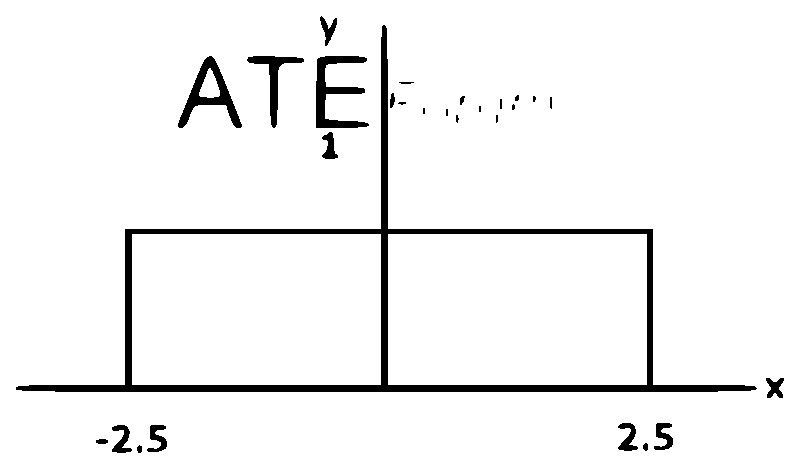
\includegraphics[scale=0.3]{fig7.eps}
%
%\begin{enumerate}[(A)]
%
%\setlength\itemsep{1em}
%
%\item $f_Y(y)=\frac{1}{5}(u(y+2.5)-u(y-2.5))$
%\item $f_Y(y)=\frac{1}{2}(\delta(y)-\delta(y-1))$
%\item $f_Y(y)=\frac{1}{4}(\delta(y+2.5)-\delta(y-2.5))+\dfrac{1}{2}\delta(y)$
%\item $f_Y(y)=\frac{1}{4}(\delta(y+2.5)-\delta(y-2.5))+\dfrac{1}{10}(u(y+2.5))-u(y-2.5)$
%
%
%\end{enumerate}

\item A system with input $x[n]$ and the ouput $y[n]$ is given as $y[n]=(sin\frac{5}{6}\pi n)x[n]$.The system is
\begin{enumerate}[(A)]

\setlength\itemsep{1em}


\item Linear,stable and invertible
\item non-linear,stable and non-invertible
\item linear,stable and non-invertible
\item linear,unstable and invertible


\end{enumerate}








%\item The 3-dB bandwidth of teh low-pass signal $e^{-t}u(t)$,where $u(t)$ is the unit step function, is given by
%
%\begin{enumerate}[(A)]
%\begin{multicols}{2}
%\setlength\itemsep{1em}
%
%\item $ \dfrac{1}{2\pi}$ Hz
%\item $ \dfrac{1}{2\pi}\sqrt{\sqrt{2}-1}$ Hz
%\item $ \infty$
%\item 1 Hz
%
%\end{multicols}
%\end{enumerate}

%
%\item The unit-step response of a system starting from rest is given by \newline $c(t)=1-e^{-2t} for t \geq 0$
%\newline The transfer function of the system is:
%
%
%\begin{enumerate}[(A)]
%\begin{multicols}{2}
%\setlength\itemsep{1em}
%
%\item $\dfrac{1}{1+2s}$
%\item $\dfrac{2}{2+s}$
%\item $\dfrac{1}{2+s}$
%\item $\dfrac{2s}{1+2s}$
%
%\end{multicols}
%\end{enumerate}


%\item A Hilbert transformer is a\\
%
%\begin{enumerate}[(A)]
%%\begin{multicols}{2}
%\setlength\itemsep{1em}
%
%\item non-linear system
%\item non-causal system
%\item time-varying system
%\item low-pass system
%
%%\end{multicols}
%\end{enumerate}

%\item The frequency response of linear,time-invariant system is given by $H(f)=\dfrac{5}{1+j10\pi f}$. The step response of the system is\\
%\begin{enumerate}[(A)]
%
%\setlength\itemsep{1em}
%
%\item $5(1-e^{-5t})u(t)$
%\item $5(1-e^{\dfrac{-t}{5}})u(t)$
%\item $\dfrac{1}{5}(1-e^{-5t})u(t)$
%\item $\dfrac{1}{5}(1-e^{\dfrac{-t}{5}})u(t)$
%
%\end{enumerate}

\item A 5-point sequence $x[n]$ is given as \newline $x[-3]=1,x[-2]=1,x[-1]=0,x[0]=5,x[1]=1.$  Let $X(e^{j\omega})$ denote the discrete -time Fourier transform of $x[n]$. The value of $\int_{-\pi}^{\pi}X(e^{j\omega})d\omega
$ is :\\
\begin{enumerate}[(A)]
\begin{multicols}{4}
\setlength\itemsep{1em}

\item 5
\item $10\pi$
\item $16\pi$
\item $5+j10\pi$

\end{multicols}
\end{enumerate}

 
\item The $z$-transform $X[z]$ of a sequence $x[n]$ is given by $X[z]=\frac{0.5}{1-2z^{-1}}$.It is given that the region of convergence of $X[z]$ includes the unit circle. The value of $x[0]$ is:\\
\begin{enumerate}[(A)]
\begin{multicols}{4}
\setlength\itemsep{1em}

\item -0.5
\item 0
\item 0.25
\item 0.5

\end{multicols}
\end{enumerate}

%\item The input and output of a continous time systems are respectively denoted by $x(t)$ and $y(t)$.Which of the following descriptions corresponds to a causal system?\\
%\begin{enumerate}[(A)]
%
%\setlength\itemsep{1em}
%
%\item $y(t)=x(t-2)+x(t+4)$
%\item $y(t)=(t-4)x(t+1)$
%\item $y(t)=(t+4)x(t-1)$
%\item $y(t)=(t+5)x(t+5)$
%
%
%\end{enumerate}


%\item The impulse response $h(t)$ of a linear time-invariant continuous time system is described by $h(t)=e^{\alpha t}u(t)+e^{\beta t}u(-t)$,where $u(t)$ denotes the unit step function, and $\alpha$ and $\beta$ are real constants.This system is stable if\\
%
%\begin{enumerate}[(A)]
%
%\setlength\itemsep{1em}
%
%\item $\alpha$ is positive and $\beta$ is positive
%\item $\alpha$ is negative and $\beta$ is negative
%\item $\alpha$ is positive and $\beta$ is negative
%\item $\alpha$ is negative and $\beta$ is positive
%
%
%\end{enumerate}

%\item A linear,time-invariant, causal continuous time system has a rational transfer function with simple poles at s=-2 and s=-4 , and one simple zero at s=-1. A unit step $u(t)$ is applied at the input of the system. At steady state, the output has constant value of 1. The impulse response of this system is\\
%\begin{enumerate}[(A)]
%
%\setlength\itemsep{1.5em}
%
%\item $[e^{-2t}+e^{-4t}]u(t)$
%\item $[-4e^{-2t}+12 e^{-4t}-e^{-t}]u(t)$
%\item $[-4e^{-2t}+12e^{-4t}]u(t)$
%\item $[-0.5e^{-2t}+1.5e^{-4t}]u(t)$
%
%\end{enumerate}


%\item The signal x(t) is described by
%\[
%	x(t)=\begin{cases}
%		1, & \text{for $-1\leq t \leq 1$}  \\
%		0, & \text{otherwise }\,.
%	\end{cases}
%\]
%\begin{enumerate}[(A)]
%\begin{multicols}{2}
%\setlength\itemsep{1em}
%
%\item $
%\pi,2\pi
%$
%\item $
%0.5\pi,1.5\pi
%$
%\item $
%0,\pi
%$
%\item $
%2\pi,2.5\pi
%$
%
%
%\end{multicols}
%\end{enumerate}

\item A discrete time linear shift-invariant system has an impulse response $h[n]$ with $h[0]=1,h[1]=-1, h[2]=-2$ and zero otherwise.The system is given an input sequence $x[n]$ with $x[0]=x[2]=\-1$, and zero otherwise. The number of nonzero samples in the output sequence $y[n]$,and the value of $y[2]$ are, respectively\\
\begin{enumerate}[(A)]
\begin{multicols}{2}
\setlength\itemsep{1em}

\item 5,2
\item 6,2
\item 6,1

\item 5,3



\end{multicols}
\end{enumerate}

\item $\{x(n)\}$ is real-valued periodic sequence with a period N. $x(n)$ and $X(k)$ form N-point.Discrete Fourier Transform (DFT) pairs. The DFT $Y(k)$ of the sequence $y(n)=\frac{1}{N}\sum_{r=0}^{N-1}x(r)x(n+r)$\\
\begin{enumerate}[(A)]

\setlength\itemsep{1em}

\item $
|X(k)|^{2}
$
\item $
\frac{1}{N}\sum_{r=0}^{N-1}X(r)*X(k+r)
$
\item $
\frac{1}{N}\sum_{r=0}^{N-1}X(r)X(k+r)
$
\item $
0
$\\


\end{enumerate}

% ec 2008 78 

\textbf{\textit{DATA FOR Q.16 AND 17}} In the following network, the switch is closed at t=$0^{-}$ and the sampling starts from t=0. The sampling frequency is 10Hz.\\

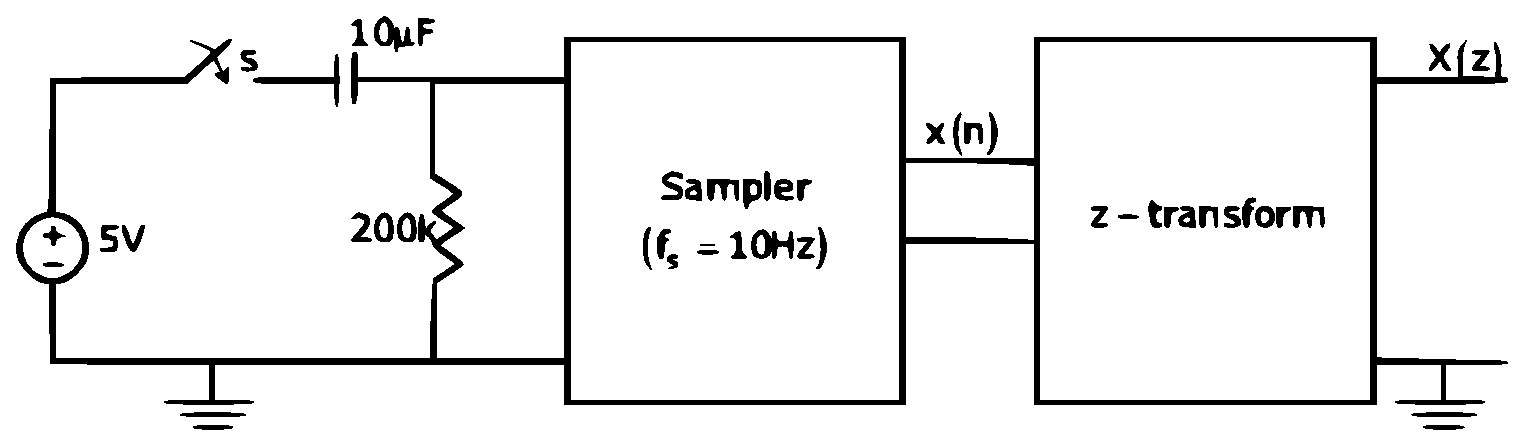
\includegraphics[scale=0.29]{fig8.eps}

\item  The samples $x(n)$ at n=0,1,2,... given by


\begin{enumerate}[(A)]

\item $5(1-e^{-0.05n})$

\item $5e^{-0.05n}$

\item $ 5(1-e^{-5n})$
\item $ 5e^{-5n}$



\end{enumerate}

\item The expression and the region of convergence of the z-transform of the sampled signal are

\begin{enumerate}[(A)]

\item $ \frac{5z}{z-e^{-5}}, |z|<e^{-5}$

\item $ \frac{5z}{z-e^{-0.05}}, |z|<e^{-0.05}$

\item $ \frac{5z}{z-e^{-5}}, |z|>e^{-0.05}$

\item  $ \frac{5z}{z-e^{-5}}, |z|>e^{-5}$



\end{enumerate}

 


%\item A function is given by $f(t)=sin^{2}t+cos2t.$ Which of the following is true ?
%
%\begin{enumerate}[(A)]
%
%\setlength\itemsep{1em}
%
%\item $f$ has frequnecy components at 0 and $\dfrac{1}{2\pi}$ Hz
%\item $f$ has frequnecy components at 0 and $\dfrac{1}{\pi}$ Hz
%\item $f$ has frequnecy components at $\dfrac{1}{2\pi}$ and $\dfrac{1}{\pi}$ Hz
%\item $f$ has frequnecy components at 0,$\dfrac{1}{2\pi}$ and $\dfrac{1}{2\pi}$ Hz
%
%
%\end{enumerate}

\item The ROC of Z-transform of the discrete time sequence $x(n)=(\frac{1}{3})^{n}u(n)-(\frac{1}{2})^{n}u(-n-1)$ is

\begin{enumerate}[(A)]
\begin{multicols}{2}
\setlength\itemsep{1em}

\item $\frac{1}{3}<|z|<\frac{1}{2}$
\item $|z|>\frac{1}{2}$
\item $|z|<\frac{1}{3}$
\item $2<|z|<3$

\end{multicols}
\end{enumerate}

\item A system with transfer function $H(z)$ has impulse response h(x) defined as h(2)=1,h(3)=-1 and h(k)=0 otherwise.Consider the following statements.
     \begin{center}
     S1: H(z) is a low pass filter\end{center} \begin{center}
     
    S2: H(z) is a FIR filter \end{center} 
     
which of the following is correct ?

\begin{enumerate}[(A)]

\setlength\itemsep{1em}

\item Only S2 is true
\item Both S1 and S2 are false.
\item Both S1 and S2 are true, and S2 is a reason for S1
\item Both S1 and S2 are true, but S2 is not a reason for S1

\end{enumerate}

%\item The Fourier series of a real periodic function has only
%
%\begin{enumerate}[(P)]
%%\begin{multicols}{2}
%\setlength\itemsep{1em}
%
%\item Cosine terms if it is even
%\item Sine terms if it is even
%\item Cosine terms if it is odd
%\item Sine terms if it is odd.
%
%%\end{multicols}
%\end{enumerate}
%Which of the above statements are correct ?
%\begin{enumerate}[(A)]
%\begin{multicols}{2}
%\setlength\itemsep{1em}
%
%\item P AND S
%\item P AND R
%\item Q AND S
%\item Q AND R
%
%\end{multicols}
%\end{enumerate}

%% ec 2009 41 pic
%\item Consider a system whose input $x$ and output $y$ are related by the equation. 
%\newline$y(t)=\int_{-\infty}^{+\infty}x(t-\tau)h(2\tau)d\tau$
%Where h(t) is shown in the graph.\\
%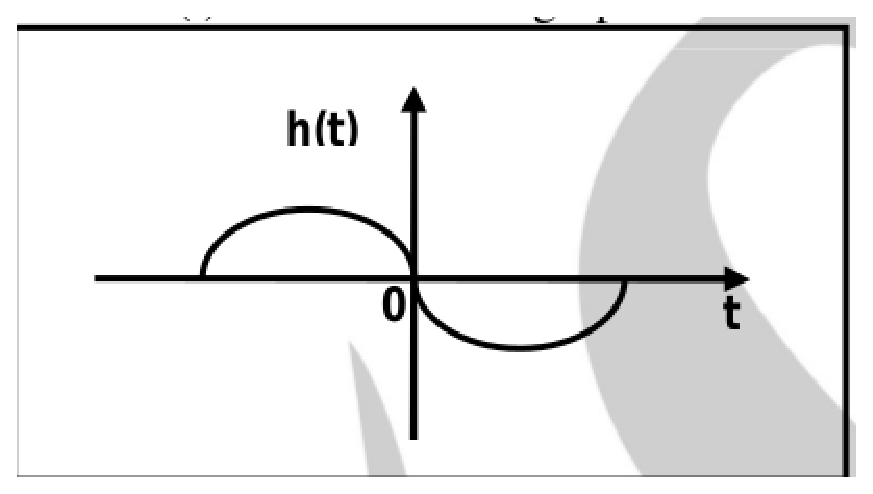
\includegraphics[scale=0.4]{fig9.eps}
%\newline Which of the following four properties are possessed by the system ?
%\newline \textbf{\textit{BIBO}}:Bounded Input gives Bounded Ouput
%\newline \textbf{\textit{Causal}}:The system is Causal.
%\newline \textbf{\textit{LP}}:The system is Lowpass.
%\newline \textbf{\textit{LTI}}:The system is Linear and Time-Invariant.\\
%\begin{enumerate}[(A)]
%\begin{multicols}{2}
%\setlength\itemsep{1em}
%
%\item Causal, LP
%\item BIBO, LTI
%\item BIBO, Causal, LTI
%\item LP,LTI
%
%\end{multicols}
%\end{enumerate}



%\item An LTI system having transfer function $\frac{s^{2}+1}{s^{2}+2s+1}$ and input $x(t)=sinx(t)$ is in steady state.The output is sampled at a rate of $\omega_w$ rad/s to obtain the final output $\{y(k)\}$. Which of the following is true ?\\
%
%\begin{enumerate}[(A)]
%
%\setlength\itemsep{1em}
%
%\item y(x) is zero for all sampling frequencies $\omega_s$
%\item y(x) is nonzero for all sampling frequencies $\omega_s$
%\item y(x) is nonzero for all sampling frequencies $\omega_s>2$, but zero for all $\omega_s<2$
%\item y(x) is zero for all sampling frequencies $\omega_s>2$, but nonzero for all $\omega_s<2$
%
%\end{enumerate}

%\item The unit step response of an under-damped second order system has steady state value of -2. Which one of the following transfer functions has these properties ?\\
%
%
%\begin{enumerate}[(A)]
%
%\setlength\itemsep{1em}
%
%\item $\dfrac{-2.24}{s^{2}+2.59s+1.12}$
%\item $\dfrac{-3.82}{s^{2}+1.91s+1.91}$
%\item $\dfrac{-2.24}{s^{2}-2.59s+1.12}$
%\item $\dfrac{-2.24}{s^{2}+2.59s+1.12}$
%
%\end{enumerate}
%ec 2010 2
%\item The trigonometric Fourier series for the waveform $f(t)$ shown below contains\\
%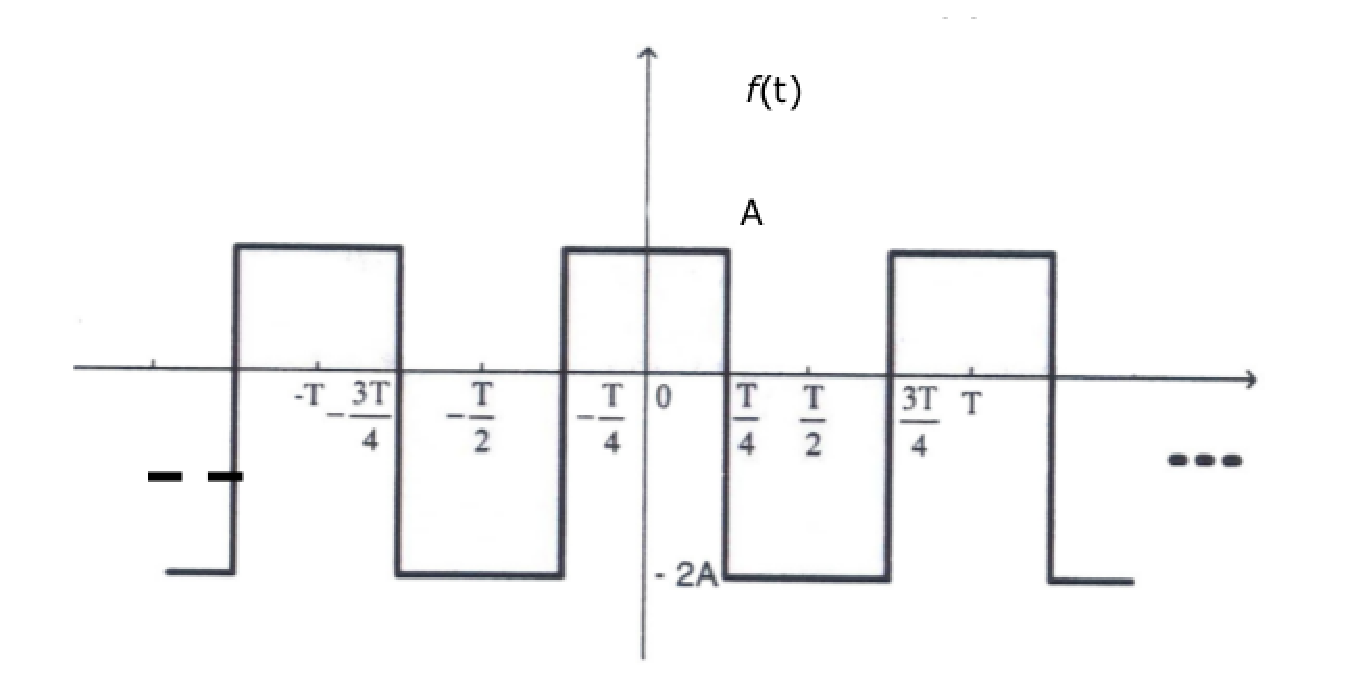
\includegraphics[scale=0.4]{fig10.eps}
%
%\begin{enumerate}[(A)]
%
%\setlength\itemsep{1em}
%
%\item only cosine terms and zero value for the dc component
%\item only cosine terms and a positive value for the dc component
%\item only cosine terms and a negative value for the dc component
%\item only sine terms and a negative for the dc component
%
%\end{enumerate}

\item Consider the z-transform $X(z)=5z^{2}+4z^{-1}+3;0<|z|<\infty$. The inverse z-transform $x[n]$

\begin{enumerate}[(A)]

\setlength\itemsep{1em}

\item $5\delta[n+2]+3\delta[n]+4\delta[n-1]$
\item $5\delta[n-2]+3\delta[n]+4\delta[n+1]$
\item $5u[n+2]+3u[n]+4u[n-1]$
\item $5u[n-2]+3u[n]+4u[n+1]$

\end{enumerate}

\item Two discrete time systems with impulse responses $h_1[n]=\delta[n-1]$ and $h_2[n]=\delta[n-2]$ are cascade. The overall impulse response of the cascaded system is

\begin{enumerate}[(A)]
\begin{multicols}{2}
\setlength\itemsep{1em}

\item $\delta[n-1]+\delta[n-2]$
\item $\delta[n-4]$
\item $\delta[n-3]$
\item $\delta[n-1]\delta[n-2]$
\end{multicols}
\end{enumerate}
%
%\item For an N-point FFT algorithm with $N=2^{m}$ which one of the following statement is TRUE?
%
%\begin{enumerate}[(A)]
%
%\setlength\itemsep{1em}
%
%\item It is not possible to construct a signal flow graph with both input and output in normal order.
%\item The number of butterflies in the $m^{th}$ stage is N/m
%\item In-place computation requires storage of only 2N node data
%\item Computation of a butterfly requires only one complex multiplication
%
%
%\end{enumerate}

%
%\item A system with transfer function $\dfrac{Y(s)}{X(s)}=\dfrac{s}{s+p}$ has an output $y(t)=cos(2t-\dfrac{\pi}{3}$ for the input signal $x(t)=p cos(2t-\dfrac{\pi}{2}$.Then, the system parameter 'p' is
%
%
%\begin{enumerate}[(A)]
%
%\setlength\itemsep{1em}
%
%\item $\sqrt{3}$
%\item $\dfrac{2}{\sqrt{3}}$
%\item $1$
%\item $\dfrac{\sqrt{3}}{2}$
%
%\end{enumerate}

%\item A continous time LTI system is described by $\dfrac{d^{2}y(t)}{dt^{2}}+4\dfrac{dy(t)}{dt}+3y(t)=2\dfrac{dx(t)}{dt}+4x(t)$
%
%\begin{enumerate}[(A)]
%
%\setlength\itemsep{1em}
%
%\item $(e^{t}-e^{3t})u(t)$
%\item $(e^{-t}-e^{-3t})u(t)$
%\item $(e^{-t}+e^{-3t})u(t)$
%\item $(e^{t}+e^{3t})u(t)$
%
%\end{enumerate}

\item The transfer function of a discrete time LTI system is given by $H(z)=\frac{2-\frac{3}{4}z^{-1}}{1-\frac{3}{4}z^{-1}+\frac{1}{8}z^{-2}}$ \newline Consider the following statements:
\newline \textbf{\textit{S1:}}The system is stable and causal for ROC:$|z|>\frac{1}{2}$
\newline \textbf{\textit{S2:}}The system is stable but not causal for ROC:$|z|<\frac{1}{4}$
\newline \textbf{\textit{S3:}}The system is neither stable nor  causal for ROC:$\frac{1}{4}<|z|<\frac{1}{2}$
\newline Which one of the following statements is valid?
\begin{enumerate}[(A)]

\setlength\itemsep{1em}

\item Both S1 and S2 are true.
\item Both S2 and S3 are true.
\item Both S1 and S3 are true.
\item S1,S2 and S3 are all true.

\end{enumerate}

%\item The Nyquist sampling rate for the signal $s(t)=\dfrac{sin(500\pi t)}{\pi t}\times \dfrac{sin(700\pi t)}{\pi t}$ is given by 
%
%\begin{enumerate}[(A)]
%\begin{multicols}{2}
%\setlength\itemsep{1em}
%
%\item 400 Hz
%\item 600 Hz
%\item 1200 Hz
%\item 1400 Hz
%\end{multicols}
%\end{enumerate}

\item A system is defined by its impulse response $h(n)=2^{n}u(n-2)$. The system is

\begin{enumerate}[(A)]
%\begin{multicols}{2}
\setlength\itemsep{1em}

\item stable and causal
\item causal but not stable
\item stable but not causal
\item unstable and non-causal
%\end{multicols}
\end{enumerate}

%\item If the unit step response of a network is $1-e^{-\alpha t}$, then its unit impulse response
%
%\begin{enumerate}[(A)]
%%\begin{multicols}{4}
%\setlength\itemsep{1em}
%
%\item $\alpha e^{-\alpha t}$
%\item $\alpha^{-1} e^{-\alpha t}$
%\item $(1-\alpha^{-1}) e^{-\alpha t}$
%\item $(1-\alpha) e^{-\alpha t}$
%%\end{multicols}
%\end{enumerate}

%\item The trigonometric Fourier series of an even function does not have the
%\begin{enumerate}[(A)]
%%\begin{multicols}{4}
%\setlength\itemsep{1em}
%
%\item dc term
%\item cosine terms
%\item sine terms
%\item odd harmonic terms
%%\end{multicols}
%\end{enumerate}

%\item An input $x(t)=e^{-2t}u(t)+\delta(t-6)$ is applied to an LTI system with impulse response $h(t)=u(t)$.The output is
%\begin{enumerate}[(A)]
%%\begin{multicols}{4}
%\setlength\itemsep{1em}
%
%\item $[1-e^{-2t}]u(t)+u(t+6)$
%\item $[1-e^{-2t}]u(t)+u(t-6)$
%\item $0.5[1-e^{-2t}]u(t)+u(t+6)$
%\item $0.5[1-e^{-2t}]u(t)+u(t-6)$
%%\end{multicols}
%\end{enumerate}

%ec 2011 40
\item Two systems $H_1(z)$ and $H_2(z)$ are connected in cascade as shown below.The overall output y(n) is the same as the input x(n) with a one unit delay. The transfer function of the second system $H_2(z)$ is\\
%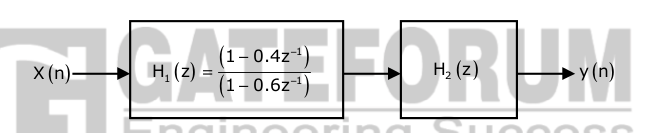
\includegraphics[scale=0.4]{fig11.eps}
{\small
\begin{equation*}
X(n) \longrightarrow \boxed{H_1(z) = \frac{1-0.4z^{-1}}{1-0.6 z^{-1}}}\longrightarrow \boxed{H_2(z)} \longrightarrow y(n)
\end{equation*}  
}

\begin{enumerate}[(A)]
\begin{multicols}{2}
\setlength\itemsep{1em}

\item $\frac{(1-0.6z^{-1})}{z^{-1}(1-0.4z^{-1})}$
\item $\frac{z^{-1}(1-0.6z^{-1})}{(1-0.4z^{-1})}$
\item $\frac{z^{-1}(1-0.4z^{-1})}{(1-0.6z^{-1})}$
\item $\frac{(1-0.4z^{-1})}{z^{-1}(1-0.6z^{-1})}$
\end{multicols}
\end{enumerate}

\item The first 6 points of the 8-point DFT of a real valued sequence are 5,1-j3,0,3-j4,0 and 3+j4. The last two points of the DFT are respectively
\begin{enumerate}[(A)]
\begin{multicols}{2}
\setlength\itemsep{1em}

\item 0,1-j3
\item 0,1+j3
\item 1+j3,5
\item 1-j3,5
\end{multicols}
\end{enumerate}

%\item The systems with impulse responses $h_1(t)$ and $h_2(t)$ are connected in cascade. Then the overall impulse response of the cascaded system is given by
%\begin{enumerate}[(A)]
%%\begin{multicols}{2}
%\setlength\itemsep{1em}
%
%\item product of $h_1(t)$ and $h_2(t)$
%\item sum of $h_1(t)$ and $h_2(t)$
%\item convolution of $h_1(t)$ and $h_2(t)$
%\item Substraction of $h_2(t)$ and $h_1(t)$
%%\end{multicols}
%\end{enumerate}


%\item A band-limited signal with a maximum frequency of 5 kHz is to be sampled. According to the sampling theorem, the sampling frequency which is not valid is
%\begin{enumerate}[(A)]
%
%\begin{multicols}{2}
%\setlength\itemsep{1em}
%
%\item 5 kHz
%\item 12 kHz
%\item 15 kHz
%\item 20 kHz
%\end{multicols}
%\end{enumerate}

%ec  2013 21
%\item Assuming zero initial condition, the response $y(t)$ of the system given below to a unit step input $u(t)$ is\\
%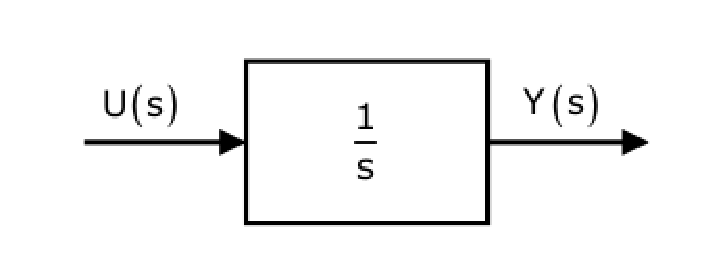
\includegraphics[scale=0.4]{fig12.eps}
%\begin{enumerate}[(A)]
%
%\begin{multicols}{2}
%\setlength\itemsep{1em}
%
%\item $u(t)$
%\item $tu(t)$
%\item $\frac{t^{2}}{2}u(t)$
%\item $e^{-t} u(t)$
%\end{multicols}
%\end{enumerate}

%\item A system is described by the differential equation $\frac{d^{2}y}{dt^{2}}+5\frac{dy}{dt}+6y(t)=x(t)$. Let x(t)  be a rectangular pulse given by\[
%	x(t)=\begin{cases}
%		1, & \text{$0<t<2$}  \\
%		0, & \text{otherwise }\,.
%	\end{cases}
%\] Assuming that $y(0)=0$ and $\frac{dy}{dt}=0$ at t=0, the Laplace transform of $y(t)$ is
%
%\begin{enumerate}[(A)]
%
%\begin{multicols}{2}
%\setlength\itemsep{1em}
%
%\item $\frac{e^{-2s}}{s(s+2)(s+3)}$
%\item $\frac{1-e^{-2s}}{s(s+2)(s+3)}$
%\item $\frac{e^{-2s}}{(s+2)(s+3)}$
%\item $\frac{1-e^{-2s}}{(s+2)(s+3)}$
%\end{multicols}
%\end{enumerate}




\item Let x[n]=x[-n]. Let X(z) be the z-transform of x[n]. If 0.5+j0.25 is a zero of X(z) then one of the following must be a zero of X(z).
\begin{enumerate}[(A)]

\begin{multicols}{2}
\setlength\itemsep{1em}

\item $0.5-j0.25$
\item $\frac{1}{0.5+j0.25}$
\item $\frac{1}{0.5-j0.25}$
\item $2+j4$
\end{multicols}
\end{enumerate}

%
%\item An FIR system is described by the system function $H(z)=1+\frac{7}{2}z^{-1}+\frac{3}{2z^{-2}}$. The system is 
%\begin{enumerate}[(A)]
%
%\begin{multicols}{2}
%\setlength\itemsep{1em}
%
%\item maximum phase
%\item minimum phase
%\item mixed phase
%\item zero phase
%\end{multicols}
%\end{enumerate}




\item The input-output relationship of a causal stable LTI system is given as $y[n]=\alpha y[n-1]+\beta x[n]$ \newline If the impulse response $h[n]$ of this system satisfies the condition $\sum_{n=0}^{\infty}h[n]=2$, the relationship between $\alpha$ and $\beta$ is
\begin{enumerate}[(A)]

\begin{multicols}{2}
\setlength\itemsep{1em}

\item $\alpha=1-\frac{\beta}{2}$
\item $\alpha=1+\frac{\beta}{2}$
\item $\alpha=2\beta$
\item $\alpha=-2\beta$
\end{multicols}
\end{enumerate}


%\item The impulse response of a system is $h(t)=tu(t)$.For an input $u(t-1)$,the output is
%\begin{enumerate}[(A)]
%
%%\begin{multicols}{2}
%\setlength\itemsep{1em}
%
%\item $\frac{t^{2}}{2}u(t)$
%\item $\frac{t\times (t-1)}{2}u(t-1)$
%\item $\frac{(t-1)^{2}}{2}u(t-1)$
%\item $\frac{t^{2}-1}{2}u(t-1)$
%%\end{multicols}
%\end{enumerate}

%\item The value of the integral $\int_{-\infty}^{+\infty} sinc^{2}(5t) dt$ is \underline{\hspace{1cm}}

%ec 2014 papr2 19
%\item Consider the periodic square wave in the figure shown.
%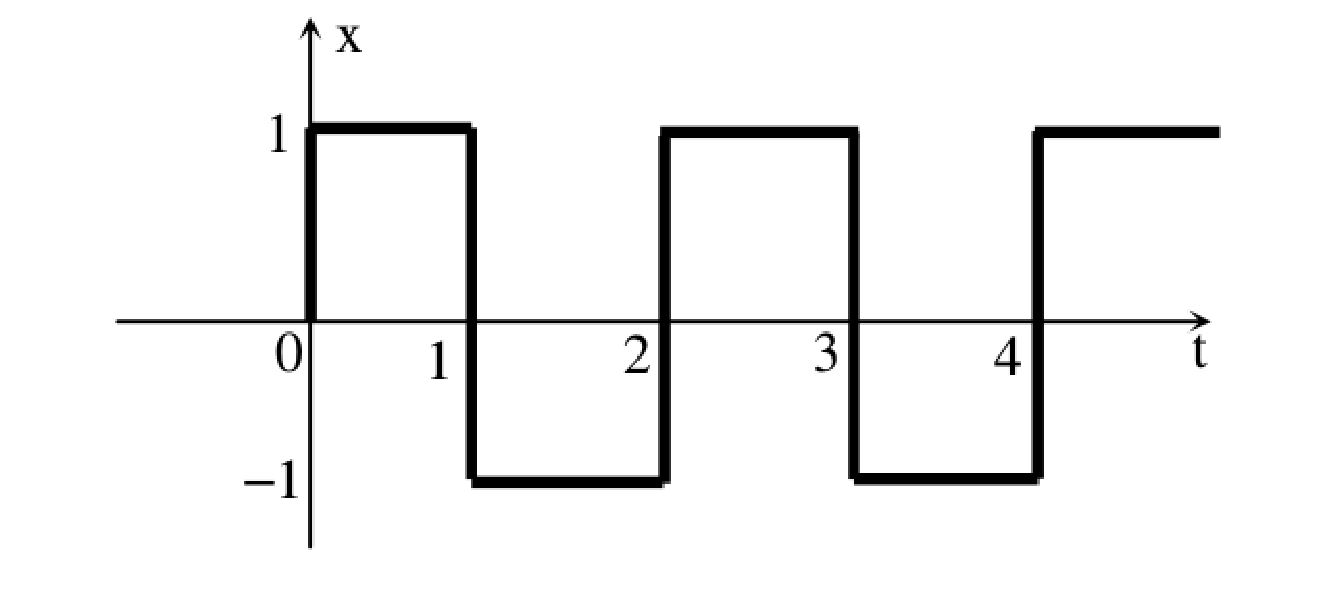
\includegraphics[scale=0.4]{fig13.eps}
%\newline The ratio of the power in the $7^{th}$ harmonic to the power in the $5^{th}$ harmonic for this waveform is closest in value to \underline{\hspace{2cm}}\\
%





% set1 2015 18
%\item The waveform of a periodic signal $x(t)$ is shown in the figure.\\
%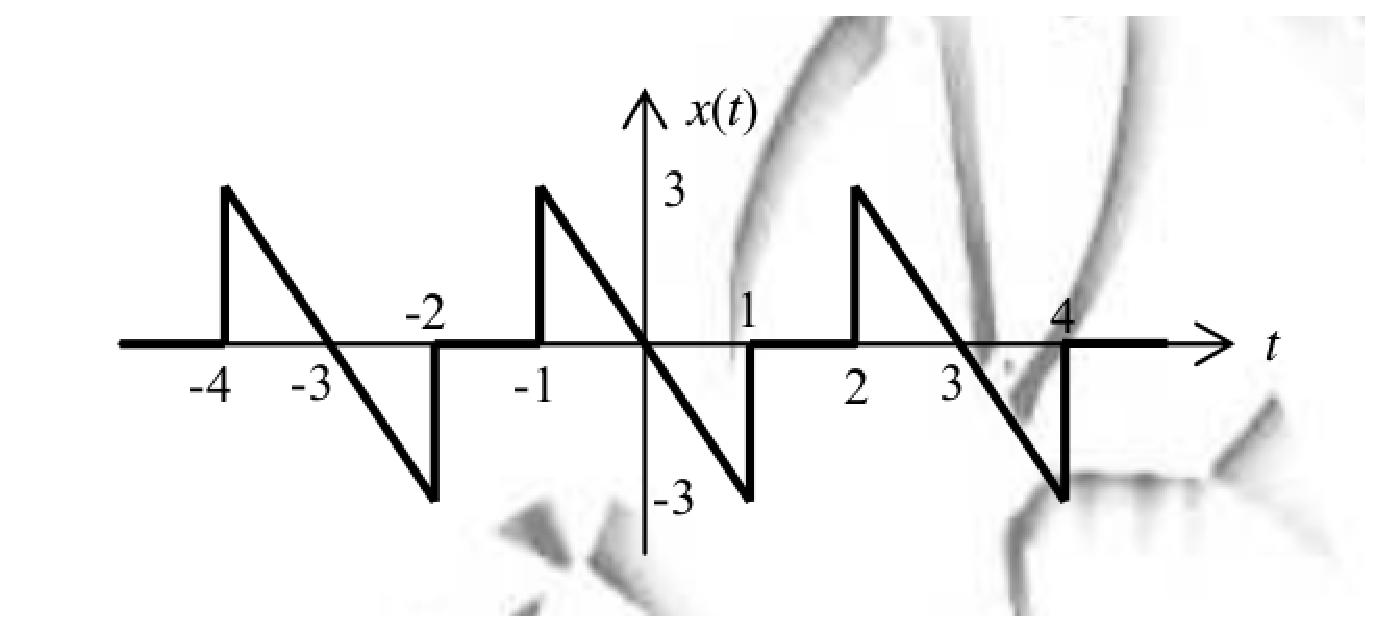
\includegraphics[scale=0.4]{fig14.eps}
%\newline A signal $g(t)$ is defined by $g(t)=x(\frac{t-1}{2})$. The average power of $g(t)$ is \underline{\hspace{2cm}}\\


%\item Consider the signal $s(t)=m(t)cos(2\pi f_c t)+\hat{m}(t)sin(2\pi f_c t)$ where $\hat{m}(t)$ denotes the Hilbert transform of $m(t)$ and the bandwidth of $m(t)$ is very small compared to $f_c$.The signal $s(t)$ is a
%
%\begin{enumerate}[(A)]
%
%%\begin{multicols}{2}
%\setlength\itemsep{1em}
%
%\item high-pass signal
%\item low-pass signal
%\item band-pass signal
%\item double sideband suppressed carrier signal
%%\end{multicols}
%\end{enumerate}





% 45 2015 set1
\item The pole-zero diagram of causal and stable discrete-time system is shown in figure. The zero at the origin has multiplicity 4. The impulse response of the system is $h[n]$. If $h[0]=1$, we can conclude\\
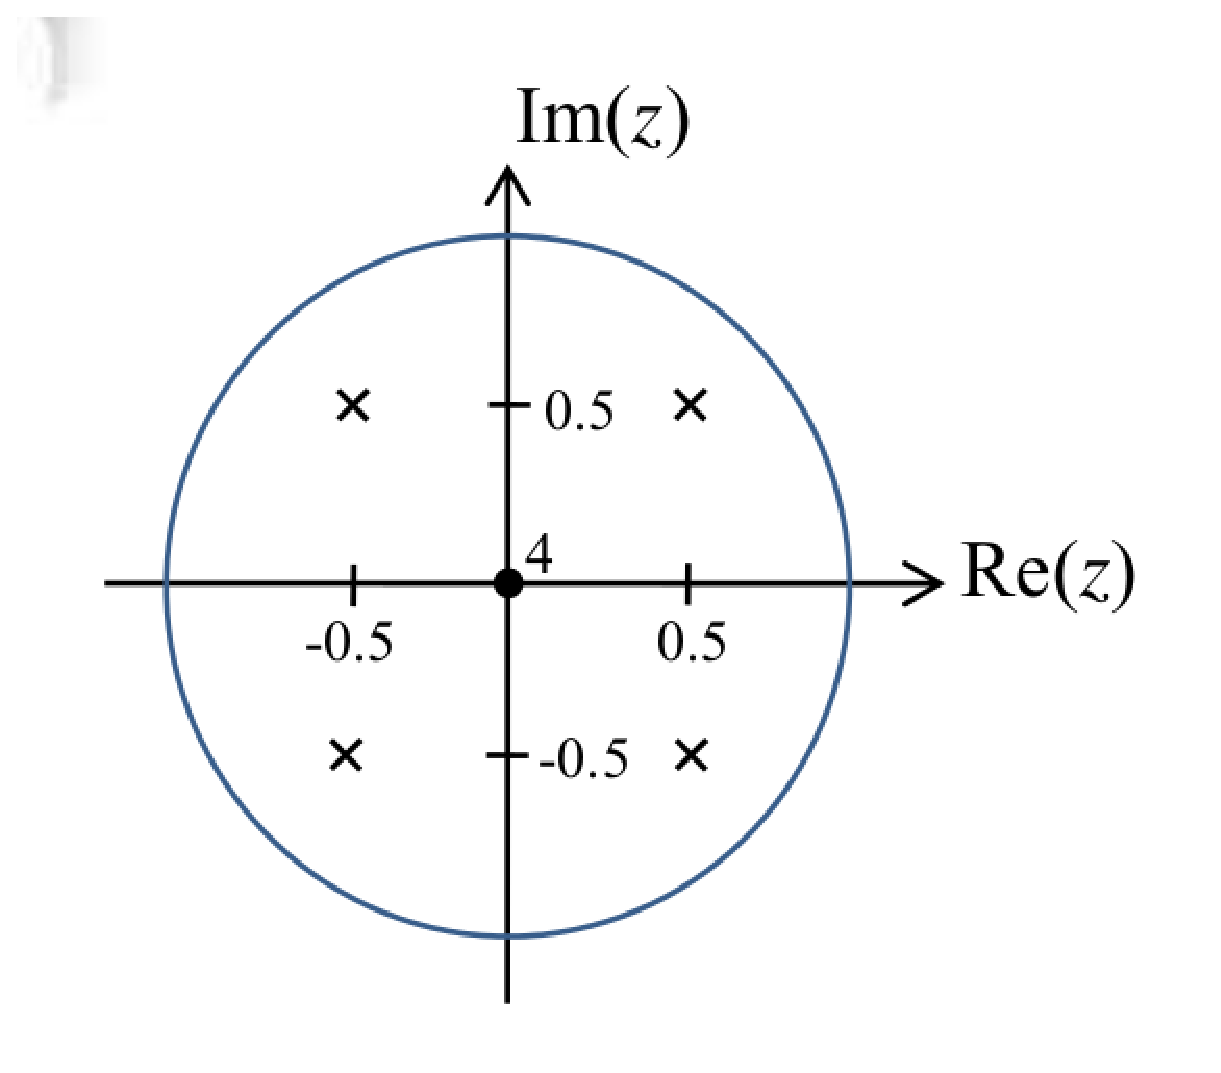
\includegraphics[scale=0.4]{fig16.eps}
\begin{enumerate}[(A)]

%\begin{multicols}{2}
\setlength\itemsep{1em}

\item $h[n]$ is real for all n
\item $h[n]$ is purely imaginary for all n
\item $h[n]$ is real for only even n
\item $h[n]$ is purely imaginary for only odd n
%\end{multicols}
\end{enumerate}




%\item A continuous-time sinusoid of frequency 33 Hz is multiplied with a periodic Dirac impulse train of frequency 46 Hz. The resulting signal is passed through an ideal analog low-pass filter with a cutoff frequency of 23 Hz. The fundamental frequency (in Hz) of the output is \underline{\hspace{2cm}}

\item Consider the signal $x[n]=6\delta [n+2]+3\delta [n+1]+8\delta[n]+7\delta[n-1]+4\delta[n-2]$. If $X(e^{j\omega})$ is the discrete-time Fourier transform of $x[n]$. Then $\frac{1}{\pi}\int_{-\pi}^{\pi}X(e^{j\omega}) sin^{2}(2\omega)d\omega$ is equal to \underline{\hspace{2cm}}

% 51 2015 set1
%\item In the system shown in Figure(a), $m(t)$ is a low-pass signal with bandwidth $W$ Hz. The frequency response of the band-pass filter $H(f)$ is shown in Figure(b). If it is described that the output signal $z(t)=10x(t)$, the maximum value of $W$ (in Hz) should be strictly less than \underline{\hspace{2cm}}\\
%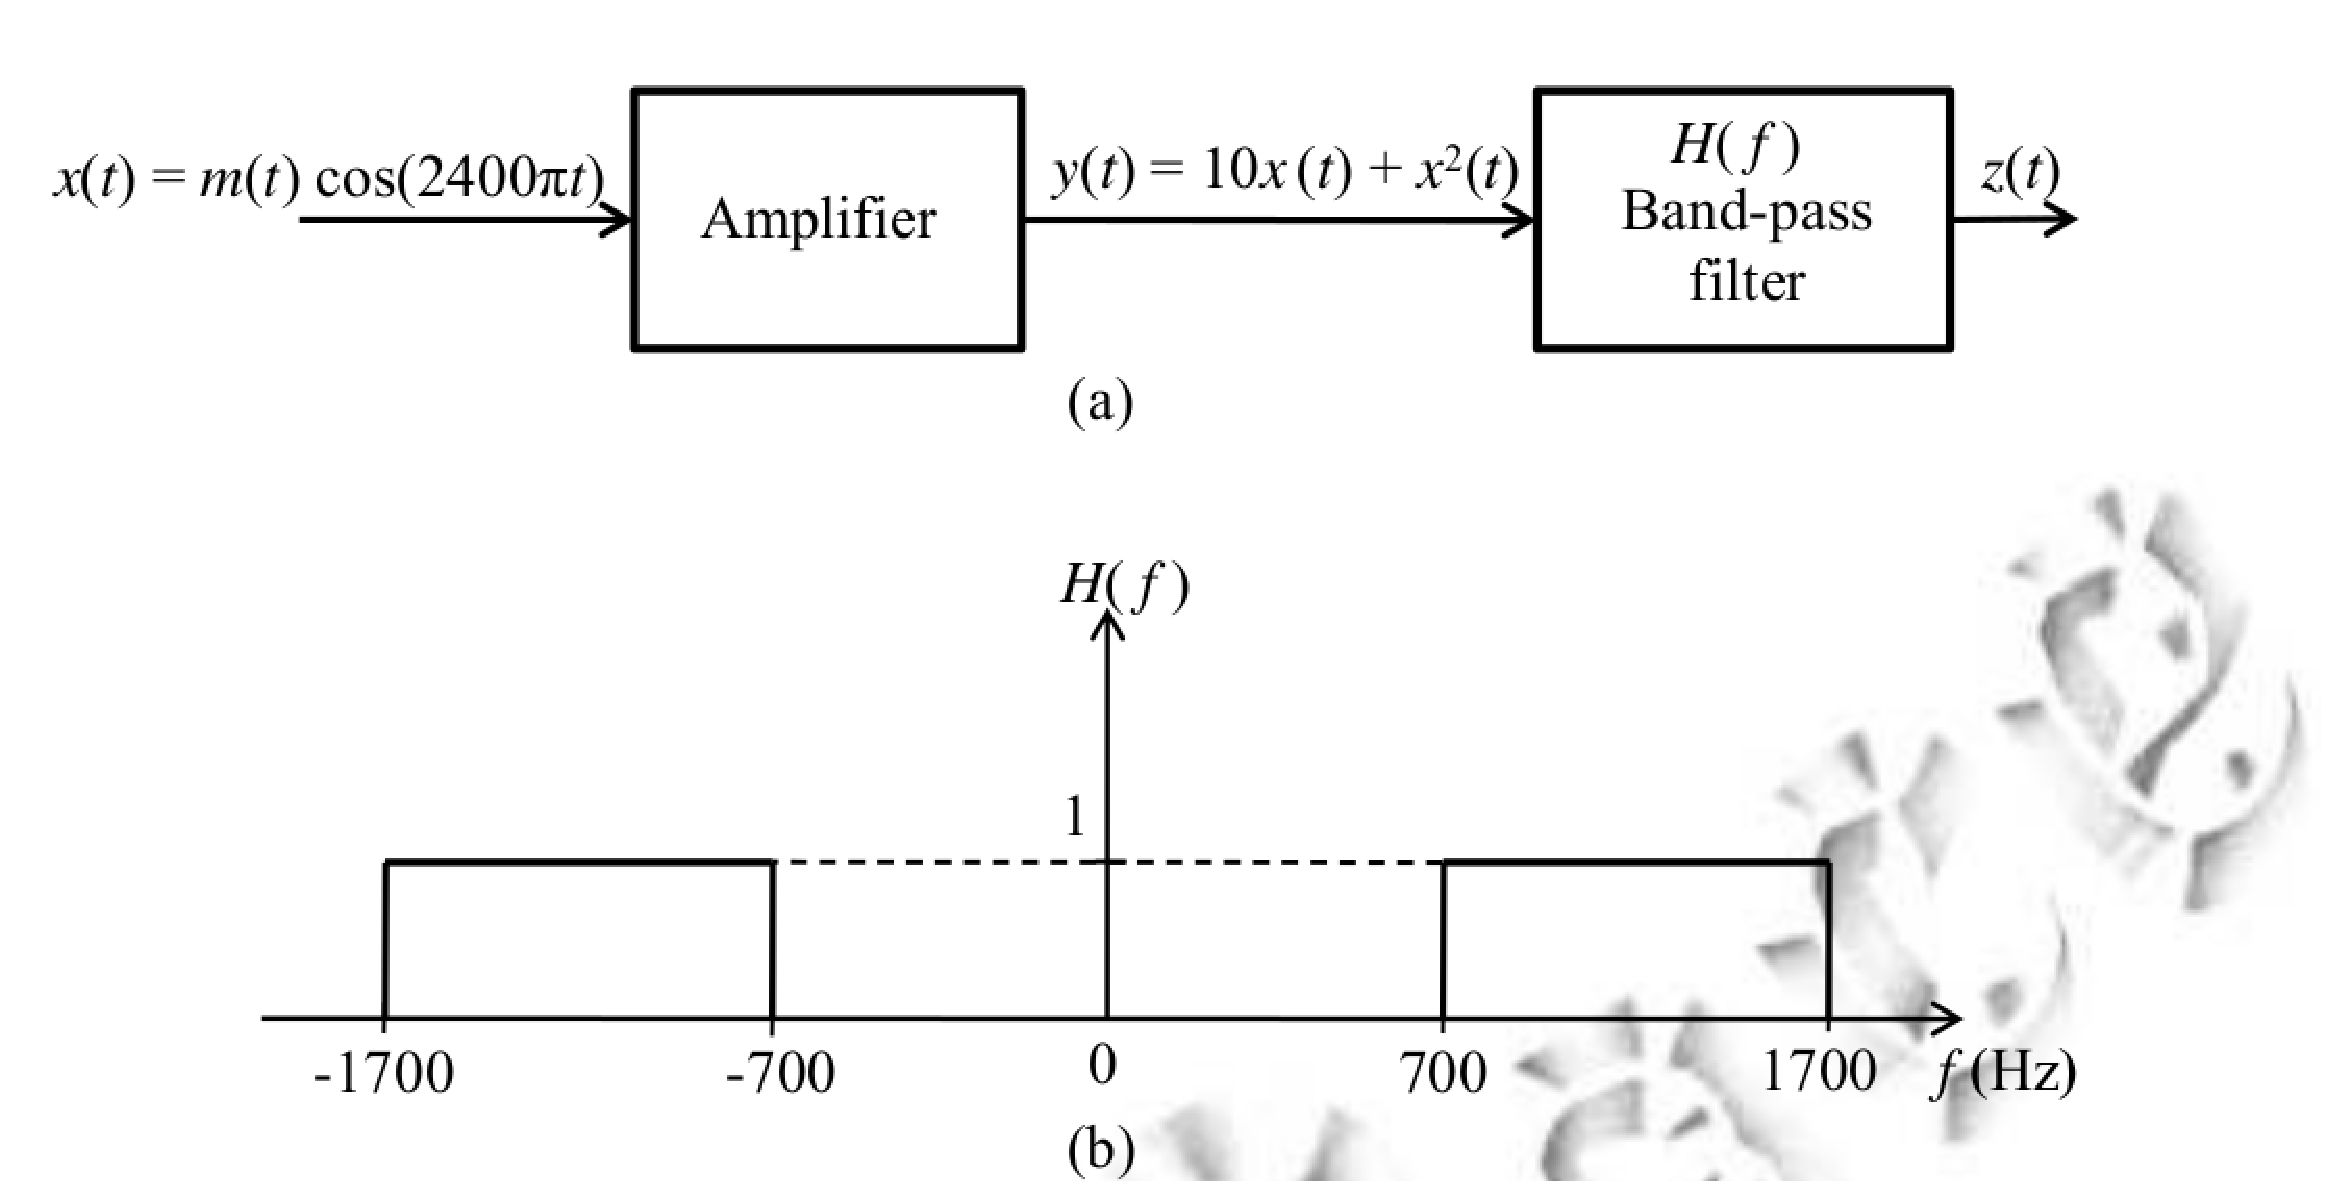
\includegraphics[scale=0.2]{fig17.eps}


%Data for \textbf{\textit{Q.108-109}} are given below.\newline
%\hspace{1em}The impulse response $h(t)$ of a linear time invariant continuous time system is given by $h(t)=e^{-2t}u(t)$, where $u(t)$ denotes the unit step function.\newline
%\item The frequency response $H(\omega)$ of this system in terms of angular frequency $\omega$ is give by $H(\omega)$ 
%
%
%
%\begin{enumerate}[(A)]
%\begin{multicols}{2}
%\setlength\itemsep{1em}
%
%\item $
%\dfrac{1}{1+j2\omega}
%$
%\item $
%\dfrac{sin(\omega)}{\omega}
%$
%\item $
%\dfrac{1}{2+j\omega}
%$
%\item $
%\dfrac{j\omega}{2+j\omega}
%$
%
%\end{multicols}
%\end{enumerate}
%
%
%
%\item The output of this system to the sinusoidal input $x(t)=2cos(2t)$ $\forall t$, is
%
%\begin{enumerate}[(A)]
%
%\setlength\itemsep{1em}
%
%\item 0
%\item $2^{-0.25}cos(2t-0.125\pi)$
%\item $2^{-0.5}cos(2t-0.125\pi)$.
%\item $2^{-0.5}cos(2t-0.25\pi)$
%
%
%\end{enumerate}
%
%\item A system described by a linear,constant coefficient, ordinary, first order differential equation has an exact solution given by $y(t)$ for $t>0$,when the forcing function is $x(t)$ and the initial condistion is $y(0)$.If one wishes to modify the system so that the solution becomes $-2y(t)$ for $t>0$, we need to
%\begin{enumerate}[(A)]
%
%%\begin{multicols}{2}
%\setlength\itemsep{2mm}
%
%\item change the initial condition to $-y(0)$ and the forcing function to $2x(t)$
%\item change the initial condition to $2y(0)$ and the forcing function to $-x(t)$
%\item change the initial condition to $j\sqrt{2y(0)}$ and the forcing function to $j\sqrt{x(t)}$
%\item change the initial condition to $-2y(0)$ and the forcing function to $-2x(t)$
%%\end{multicols}
%\end{enumerate}

% 44 2015 set1
\item For the discrete-time shown in the figure, the poles of the system transfer function are located at
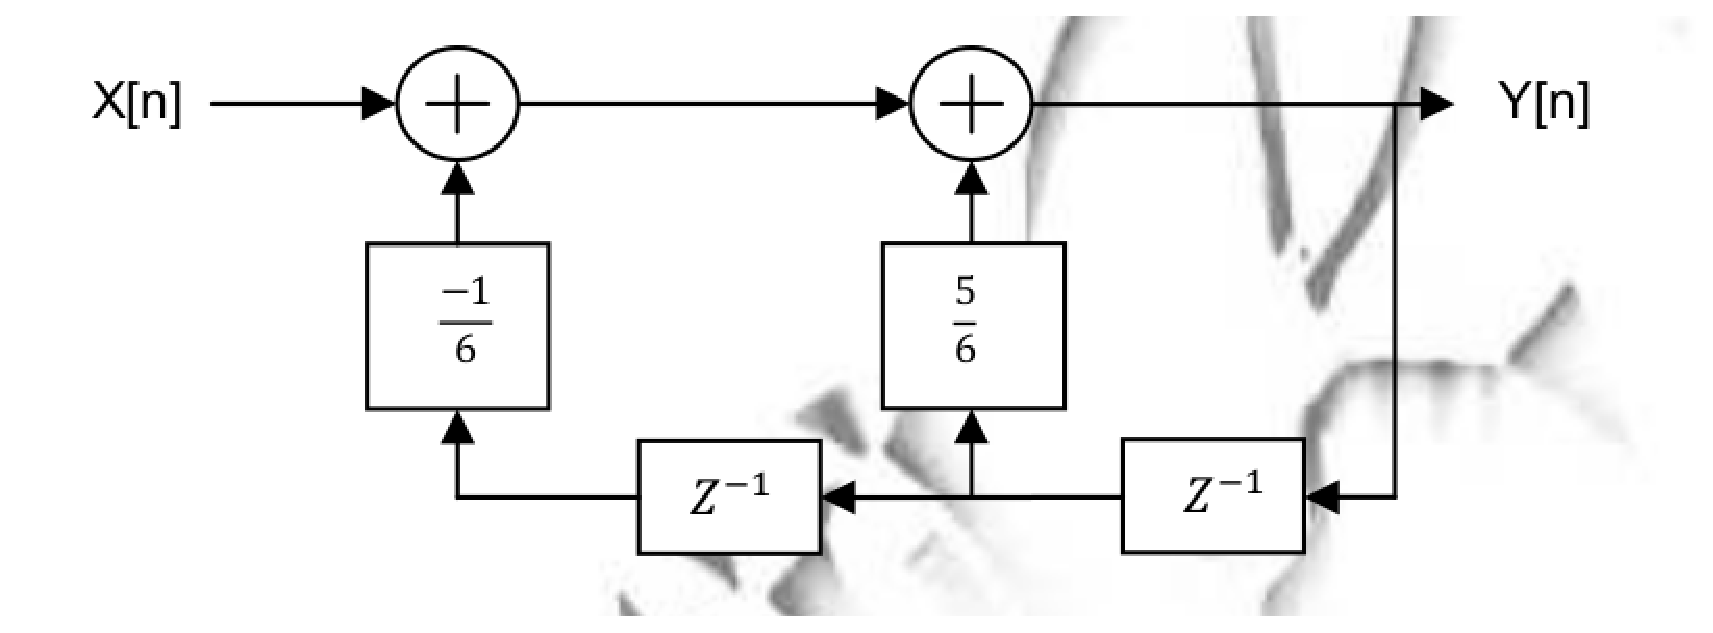
\includegraphics[scale=0.3]{fig15.eps}
\begin{enumerate}[(A)]
\begin{multicols}{2}
\setlength\itemsep{1em}

\item $2,3$
\item $\frac{1}{2},3$
\item $\frac{1}{2},\frac{1}{3}$
\item $2,\frac{1}{3}$
\end{multicols}
\end{enumerate}

%ec paper 2014 52
%\item In the figure,$M(f)$ is the Fourier transform of the message signal,$m(t)$ where A=100 Hz and B=40 Hz. Given $v(t)=cos(2\pi f_c t)$ and $w(t)=cos(2\pi (f_c +A))$, where $f_c > A$ The cutoff frequencies of the both filters are \underline{\hspace{2cm}} $f_c$\\
%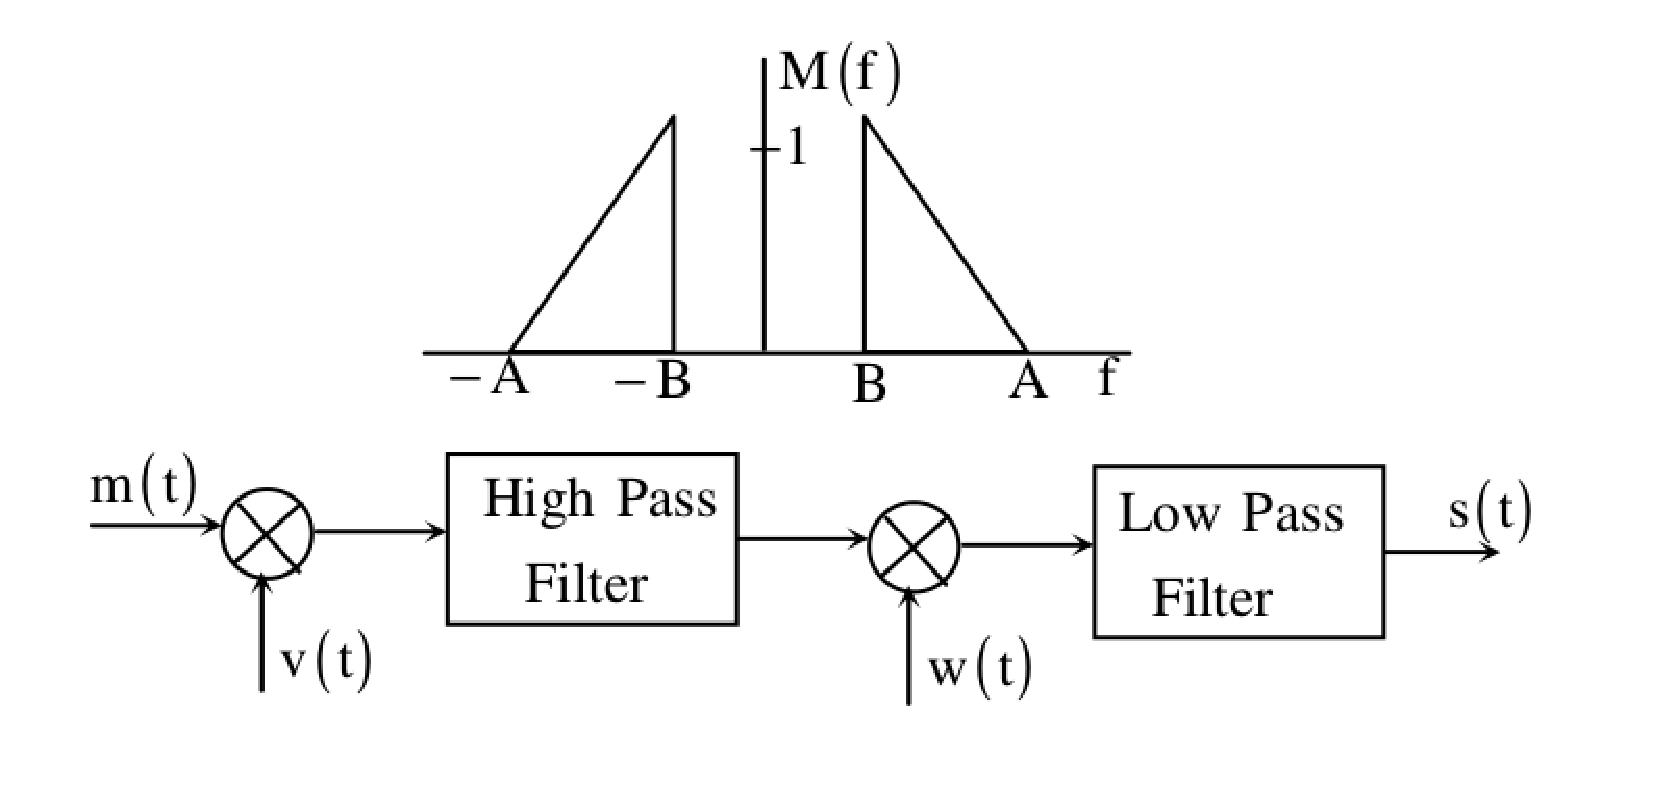
\includegraphics[scale=0.3]{fig18.eps}


%\item The result of the convolution $x(-t)*\delta(-t-t_0)$ is
%\begin{enumerate}[(A)]
%
%\begin{multicols}{2}
%\setlength\itemsep{1em}
%
%\item $x(t+t_0)$
%\item $x(t-t_0)$
%\item $x(-t+t_0)$
%\item $x(-t-t_0)$
%\end{multicols}
%\end{enumerate}


\item The DFT of vector $[a\hspace{3mm}b\hspace{3mm}c\hspace{3mm}d]$ is the vector $[\alpha \hspace{3mm}\beta \hspace{3mm}\gamma \hspace{3mm} \delta]$.Consider the product \newline $[p\hspace{3mm}q\hspace{3mm}r\hspace{3mm}s]=[a\hspace{3mm}b\hspace{3mm}c\hspace{3mm}d] \begin{bmatrix}
a & b & c & d \\
d & a & b & c \\
c & d & a & b\\
b & c & d & a
\end{bmatrix}$ 
\newline The DFT of the vector $[p\hspace{3mm}q\hspace{3mm}r\hspace{3mm}s] $ is a scaled version of \\
\begin{enumerate}[(A)]

%\begin{multicols}{2}
\setlength\itemsep{1em}

\item $[\alpha^{2} \hspace{3mm}\beta^{2} \hspace{3mm}\gamma^{2} \hspace{3mm} \delta^{2}]$
\item $[\sqrt{\alpha} \hspace{3mm}\sqrt{\beta} \hspace{3mm}\sqrt{\gamma} \hspace{3mm}\sqrt{ \delta}]$
\item $[\alpha + \beta \hspace{3mm}\beta + \delta \hspace{3mm}\gamma + \delta \hspace{3mm} \gamma + \alpha]$
\item $[\alpha \hspace{3mm}\beta \hspace{3mm}\gamma \hspace{3mm} \delta]$
%\end{multicols}
\end{enumerate}

\item Two sequences $[a\hspace{3mm}b\hspace{3mm}c]$ and $[A \hspace{3mm}B \hspace{3mm}C]$ are related as  \newline $\begin{bmatrix}
A\\
B \\
C
\end{bmatrix}=\begin{bmatrix}
1 & 1 & 1\\
1 & W^{-1}_3 & W^{-2}_3 \\
1 & W^{-2}_3 & W^{-4}_3
\end{bmatrix}\begin{bmatrix}
a\\
b \\
c
\end{bmatrix} $ Where $W_3=e^{j\frac{2\pi}{3}}$ \newline If another sequence $[p\hspace{3mm}q\hspace{3mm}r]$ is derived as \newline
$\begin{bmatrix}
p\\
q \\
r
\end{bmatrix}=\begin{bmatrix}
1 & 1 & 1\\
1 & W^{1}_3 & W^{2}_3 \\
1 & W^{2}_3 & W^{4}_3
\end{bmatrix} \begin{bmatrix}
1 & 0 & 0\\
0 & W^{2}_3 & 0 \\
0 & W^{4}_3 & 0
\end{bmatrix}\begin{bmatrix}
\frac{A}{3} \vspace{2mm}\\
\frac{B}{3} \vspace{2mm}\\
\frac{C}{3}
\end{bmatrix} $ 
\newline Then the relationship between the sequences $[p\hspace{3mm}q\hspace{3mm}r]$ and $[a\hspace{3mm}b\hspace{3mm}c]$\\
%\begin{multicols}{2}
\setlength\itemsep{1em}
\begin{enumerate}


\item $[p\hspace{3mm}q\hspace{3mm}r]=[b\hspace{3mm}a\hspace{3mm}c]$
\item $[p\hspace{3mm}q\hspace{3mm}r]=[b\hspace{3mm}c\hspace{3mm}a]$
\item $[p\hspace{3mm}q\hspace{3mm}r]=[c\hspace{3mm}a\hspace{3mm}b]$
\item $[p\hspace{3mm}q\hspace{3mm}r]=[c\hspace{3mm}b\hspace{3mm}a]$
%\end{multicols}
\end{enumerate}

\item Let $h[n]$ be the impulse response of a discrete-time linear time invariant (LTI) filter. The impulse response is given by $h[0]=\frac{1}{3};h[1]=\frac{1}{3};h[2]=\frac{1}{3}$ and $h[n]=0$ for $n<0$ and $n>0$.\newline Let $H(\omega)$ be the discrete-time Fourier transform (DTFT) of $h[n]$,where $\omega$ is the normalized angular frequency in radians. Given that $H(\omega_0)=0$ and $0<\omega < \pi$, the value of $w_0$ (in radians) is equal to \underline{\hspace{2cm}}


\item A discrete-time signal $x[n]=\delta[n-3]+2\delta[n-5]$ has $z-$transform $X(z)$. If $Y(z)=X(-z)$ is the $z-$ transform of another signal $y[n]$, then

\begin{enumerate}[(A)]
\begin{multicols}{2}
\setlength\itemsep{1em}

\item $y[n]=x[n]$
\item $y[n]=x[-n]$
\item $y[n]=-x[n]$
\item $y[n]=-x[-n]$

\end{multicols}
\end{enumerate}

\item The 4-point Discrete Fourier Transform (DFT) of a discrete time sequence {1,0,2,3} is\\
\begin{enumerate}[(A)]

\setlength\itemsep{1em}

\item $[0,-2+2j,2,-2-2j]$
\item $[2,2+2j,6,-2-2j]$
\item $[6,1-3j,2,1+3j]$
\item $[6,-1+3j,0,-1-3j]$

\end{enumerate}

\end{enumerate}


\end{document}
